
%% 
%% Copyright 2007-2025 Elsevier Ltd
%% 
%% This file is part of the 'Elsarticle Bundle'.
%% ---------------------------------------------
%% 
%% It may be distributed under the conditions of the LaTeX Project Public
%% License, either version 1.3 of this license or (at your option) any
%% later version.  The latest version of this license is in
%%    http://www.latex-project.org/lppl.txt
%% and version 1.3 or later is part of all distributions of LaTeX
%% version 1999/12/01 or later.
%% >
%% The list of all files belonging to the 'Elsarticle Bundle' is
%% given in the file `manifest.txt'.
%% 
%% Template article for Elsevier's document class `elsarticle'
%% with numbered style bibliographic references
%% SP 2008/03/01
%% $Id: elsarticle-template-num.tex 272 2025-01-09 17:36:26Z rishi $
%%
\documentclass[preprint,12pt]{elsarticle}

%% Use the option review to obtain double line spacing
%% \documentclass[authoryear,preprint,review,12pt]{elsarticle}

%% Use the options 1p,twocolumn; 3p; 3p,twocolumn; 5p; or 5p,twocolumn
%% for a journal layout:
%% \documentclass[final,1p,times]{elsarticle}
%% \documentclass[final,1p,times,twocolumn]{elsarticle}
%% \documentclass[final,3p,times]{elsarticle}
%% \documentclass[final,3p,times,twocolumn]{elsarticle}
%% \documentclass[final,5p,times]{elsarticle}
%% \documentclass[final,5p,times,twocolumn]{elsarticle}

%% For including figures, graphicx.sty has been loaded in
%% elsarticle.cls. If you prefer to use the old commands
%% please give \usepackage{epsfig}

%% The amssymb package provides various useful mathematical symbols
\usepackage{amssymb}
\usepackage{tabularx} % Asegúrate de tener esto en el preámbulo
\usepackage[hidelinks]{hyperref}
\usepackage{tikz}
\usetikzlibrary{positioning, arrows.meta, shapes.geometric}


%% The amsmath package provides various useful equation environments.
\usepackage{makecell}
\usepackage{float}
\usepackage{amsmath}
\usepackage{url}
\usepackage{comment}
\usepackage{xcolor} 
%% The amsthm package provides extended theorem environments
%% \usepackage{amsthm}

%% The lineno packages adds line numbers. Start line numbering with
%% \begin{linenumbers}, end it with \end{linenumbers}. Or switch it on
%% for the whole article with \linenumbers.
%% \usepackage{lineno}

\journal{Biofuels}

\begin{document}

\begin{frontmatter}

%% Title, authors and addresses

%% use the tnoteref command within \title for footnotes;
%% use the tnotetext command for theassociated footnote;
%% use the fnref command within \author or \affiliation for footnotes;
%% use the fntext command for theassociated footnote;
%% use the corref command within \author for corresponding author footnotes;
%% use the cortext command for theassociated footnote;
%% use the ead command for the email address,
%% and the form \ead[url] for the home page:
%% \title{Title\tnoteref{label1}}
%% \tnotetext[label1]{}
%% \author{Name\corref{cor1}\fnref{label2}}
%% \ead{email address}
%% \ead[url]{home page}
%% \fntext[label2]{}
%% \cortext[cor1]{}
%% \affiliation{organization={},
%%             addressline={},
%%             city={},
%%             postcode={},
%%             state={},
%%             country={}}
%% \fntext[label3]{}

\title{Computational Modeling of the Combustion Reaction Kinetics of the Oil Palm's Empty Fruit Bunch and Mesocarp Fiber}

%% use optional labels to link authors explicitly to addresses:
%% \author[label1,label2]{}
%% \affiliation[label1]{organization={},
%%             addressline={},
%%             city={},
%%             postcode={},
%%             state={},
%%             country={}}
%%
%% \affiliation[label2]{organization={},
%%             addressline={},
%%             city={},
%%             postcode={},
%%             state={},
%%             country={}}
\author[label1]{Arias-Guerrero D.A.}
\author[label1]{Castillo-Hernández M.}
\author[label1]{Mayorga-Guzmán J.D.}
\author[label1]{Bayona-Roa, C.A.\corref{cor1}\fnref{orc4}}

\affiliation[label1]{organization={Departamento de Ingeniería Industrial, Facultad de Ingeniería, Pontificia Universidad Javeriana},%Department and Organization 
            city={Bogotá},
            country={Colombia}}

\cortext[cor1]{Corresponding author}
\ead{ca_bayonar@javeriana.edu.co}
\fntext[orc4]{ORCID: 0000-0001-9508-1779}
\ead[url]{https://orcid.org/0000-0001-9508-1779}
% Abstract
\begin{abstract}
%% Text of abstract
Empty Fruit Bunch (EFB) and Palm Mesocarp Fiber (PMF) are abundant by-products of palm-oil milling whose energetic valorisation is limited by high moisture and corrosive ash constituents (K, Cl).  Using a computational model developed in Python and solved with the Livermore Solver for Ordinary Differential Equations with Automatic method switching algorithm, this study presents a moisture-free, mass- and energy-balanced kinetic framework that predicts the time-resolved combustion behavior of both biomasses, thereby strengthening the reproducibility and transparency of the modeling framework. The kinetic model tracks the consumption of elemental species and formation of combustion products, calibrated with data from the NIST Chemical Kinetics Database. The model accurately reproduces the low-heating-value energy releases reported in the literature—147.11 MJ for EFB and 158.27 MJ for PMF—while additionally resolving transient species profiles, heat-release rates and combustion-power curves. Simulations reveal that EFB attains its maximum heat release at an Air to Fuel Ratio $\approx$ 13 \% lower than PMF, yet still delivers greater boiler-usable enthalpy after accounting for moisture-free energy balance. Our results demonstrate that rigorous physicochemical characterisation combined with detailed chemical kinetics provides a reliable, transferable toolset for designing next-generation biomass boilers and unlocking the energy potential of agro-industrial residues such as EFB.

\end{abstract}





%% Graphical abstract
\begin{graphicalabstract}
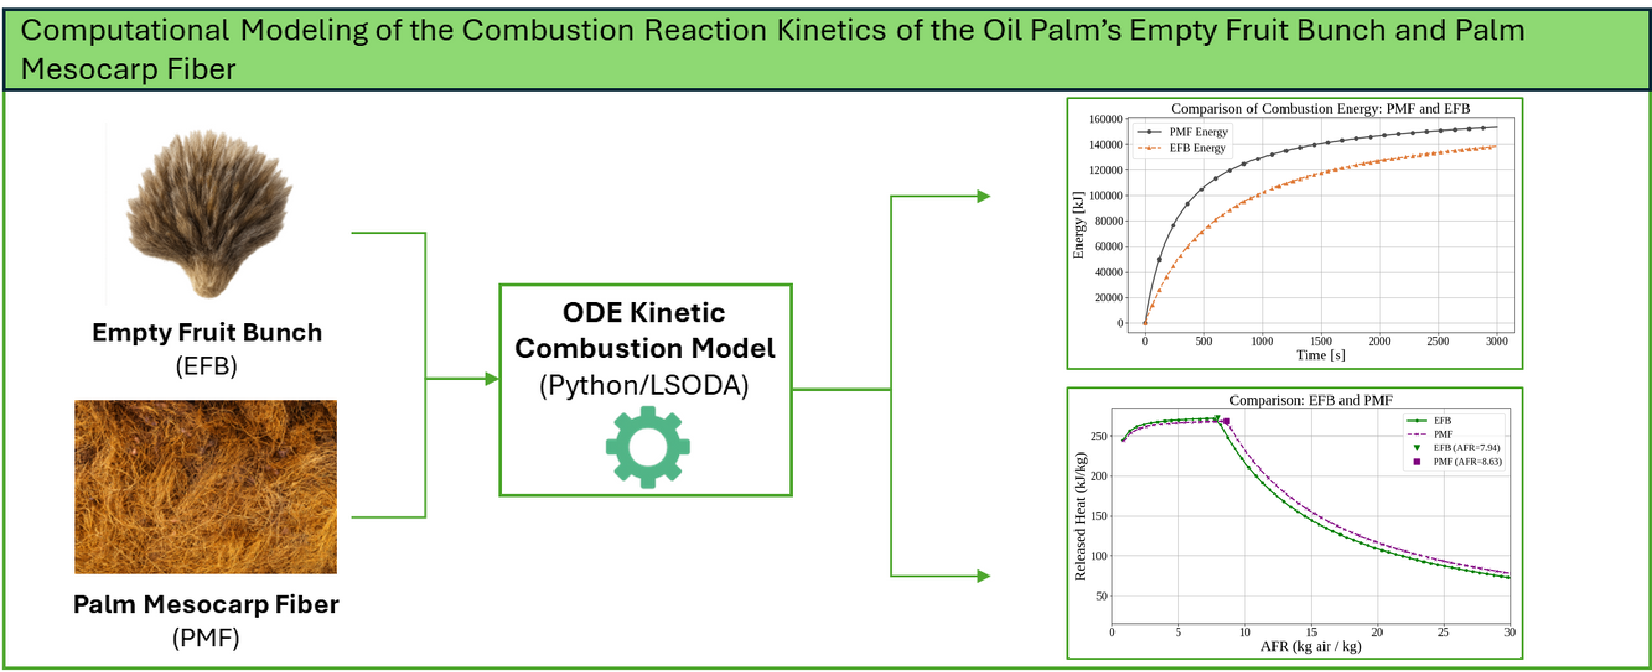
\includegraphics[width=\textwidth,trim={0 0 0 1.5cm},clip]{FIGURES/graphicalabstractPDF.pdf}
\end{graphicalabstract}


%%Research highlights
\begin{highlights}
\item Build ODE-based kinetic model for EFB and PMF combustion

\item Derive oxygen demand and optimum AFR from elemental stoichiometry

\item Python + LSODA predicts time-resolved species, heat-release and power curves

\item EFB reaches peak heat release at $\approx$ 13 \% lower AFR than PMF in air-limited firing

\item Moisture-free energy balance shows EFB yields more boiler-usable enthalpy than PMF

\end{highlights}

%% Keywords
\begin{keyword}
%% keywords here, in the form: keyword \sep keyword
Combustion\sep Empty Fruit Bunch (EFB)\sep Palm Mesocarp Fiber (PMF) \sep Reaction Kinetics\sep Combustion Modeling\sep Biomass Boilers
%% PACS codes here, in the form: \PACS code \sep code

%% MSC codes here, in the form: \MSC code \sep code
%% or \MSC[2008] code \sep code (2000 is the default)

\end{keyword}

\end{frontmatter}

%%%%%%%%%%%%%%%%%%%%%%%%%%%%%%%%%%%%%%%%%%%%%%%%%%%%%%%
% ----------------- INTRODUCTION --------------------
\section{Introduction}\label{intro}
Palm oil has become the world’s most important vegetable oil, with global output exceeding $\approx$ 78 million tons in 2023, driven chiefly by Indonesia and Malaysia, which together supply more than four-fifths of the total \cite{FAOSTAT2024,USDA2024}. Rapid acreage expansion is also occurring in emerging producer regions such as Latin America and sub-Saharan Africa, motivated by biofuel mandates, export demand and rural-development policies. \\

%Within Latin America, Colombia stands as the leading palm oil producer and ranks fourth globally, with a total output of approximately 1.8 million tons of crude palm oil in 2023, derived from the processing of around 8.3 million tons of Fresh Fruit Bunches (FFB) \cite{Fedepalma2023}. This agro-industrial activity spans nearly 600 thousand hectares of cultivated land across the country \cite{Agronet}. \\

The milling process simultaneously generates large quantities of lignocellulosic residues—chiefly Empty Fruit Bunch (EFB) and Palm Mesocarp Fiber (PMF)—whose energetic valorisation can improve both the economic and environmental performance of the industry worldwide. Among these, EFB account for approximately 20\% of the FFB weight, followed by PMF at 13\% and Palm Kernel Shells (PKS) at 4\% \cite{BayonaRaquis}, as depicted in Figure~\ref{fig:mi_imagen}. These by-products represent a significant waste, yet less than 10\% of EFB and PMF are currently used for energy or industrial purposes \cite{Fedepalma2023}.\\

\begin{figure}[h]
    \centering
    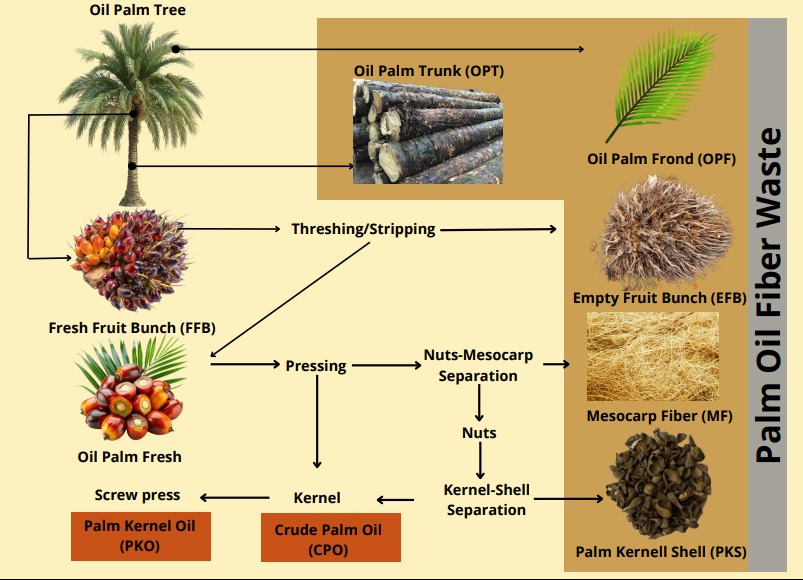
\includegraphics[width=0.9\textwidth]{FIGURES/Diagramatesis (1).jpeg}
    \caption{Main biomass residues generated in the palm oil industry.}
    \label{fig:mi_imagen}
\end{figure}

Despite its high carbon content and energy potential, EFB is often underutilized as a fertilizer after it is buried openly, leading to material loss and contributing to environmental pollution. This uncontrolled practice results in the emission of greenhouse gases such as methane, which has a global warming potential over 80 times greater than that of carbon dioxide over a 20 year horizon \cite{NacionesUnidasMetano}. In response, the exploitation of EFB in energy demanding processes is proposed.\\

Recent studies have shown that partially replacing PMF (the primary biofuel currently used in industrial boilers for energy generation in oil palm industries) with EFB can lead to a 28,81\% increase in energy potential and fulfill a cycle process of energy production \cite{BayonaRaquis}. Moreover, this substitution would enable the reallocation of PMF to value-added applications such as paper production and structural enhancement of recycled cardboard, due to its high cellulose content \cite{WanRosli2011, Angarita2009}. \\

To examine the viability of this substitution and assess the feasibility of using EFB as an alternative biofuel, understanding its chemical potential with the Low Heating Values (LHV) and kinetics (composition over time) is crucial, as these factors directly influence the energy yield and combustion behavior. A higher LHV indicates greater energy content per unit mass, while favorable kinetics ensure efficient and stable conversion during combustion. Using the LHV is the first possible model in early-stage boiler design or adaptation. Nonetheless, it is limited to quantify released thermal energy and no information about combustion gases composition can be obtained. On the other hand, combustion kinetics models of EFB is able to predict the deposition of alkali metals and chlorine, and the detailed chemical species distribution in the exhaust gases. \\%Also a modified SIR (Susceptible-Infected-Recovered) framework (originally developed for modeling epidemiological dynamics) is adapted here to simulate biomass combustion processes and evaluate the transformation of fuel elements into combustion products over time.\\

Previous studies on biomass combustion modeling have focused on Thermo Gravimetric Analysis (TGA) as the primary method for deriving kinetic parameters \cite{Khan2023}. Some works have applied the Coats–Redfern method to TGA and Derivative Thermogravimetry (DTG) data from oil palm residues to fit multi-stage decomposition models and calculate activation energies for different stages \cite{Ninduangdee2015, Jia2021}. Others have combined TGA with Differential Scanning Calorimetry (DSC) to derive thermal degradation profiles and adjust parallel reaction schemes for palm oil by-products \cite{GarciaNunez2006}. Although these methods offer detailed insights into thermal decomposition, they rely on fixed laboratory conditions, are not easily adaptable to iterative system-scale analysis, and require extensive recalibration for each scenario.\\

More complex kinetic approaches have also been developed, including detailed reaction networks of biomass pyrolysis or combustion \cite{Dhahak2021, Ranzi2013}. Those models can involve hundreds of elementary reactions and are often constructed for wood or municipal solid waste, as in \cite{Luo2019, Frank2014}. While accurate, such models require high computational effort and extensive chemical data, making them less feasible for practical, early-stage boiler design or adaptation to diverse fuels. Other works have employed empirical kinetics combined with CFD or simplified reactor models to simulate ignition and burnout phases \cite{Silva2023, Navarrete2017}, but without resolving species evolution over time or applying the method to oil palm biomass. A recent example of empirical kinetic modeling that prioritizes simplicity and curve fitting over mechanistic detail is presented in \cite{Varhegyi2020}, though it does not address time-resolved species profiles or specific applications for palm biomass.\\

By now, no previous study has developed a combustion model capable of simulating the temporal evolution of reactants and products for oil palm EFB and PMF. Most published works for these biomass either focus on fuel characterization, heating value, or static equilibrium outputs. Even existing models for EFB gasification \cite{OilPalmRachisGasification, Ramos2017} do not resolve the dynamic behavior of species concentrations during the reaction process. As a result, there is a lack of tools capable of supporting time-dependent combustion diagnostics for this biomass in boiler systems.\\

In contrast, the model proposed in this study introduces an accessible method to simulate EFB and PMF combustion, for easier numerical resolution and visualization of the results (in Python). It uses a system of coupled ordinary differential equations derived from mass balance principles for each biomass. While the LHV of the biomass is used to validate the final energy output, the model allows for the resolution of species evolution, combustion duration, and conversion completeness. Additionally, it supports a dynamic energy and power analysis based on the simulated temporal profiles and a defined combustion chamber volume, enabling thermochemical evaluation throughout the reaction. The model can also be extended to perform parametric Air-Fuel Ratio (AFR) analysis to identify the value that maximizes thermal energy release for each biomass, facilitating direct fuel comparisons under standardized conditions. This structure offers insight into reactant depletion, intermediate formation, and product stabilization (information not captured by static models) inside the combustion chamber. Moreover, it permits integration into future studies on flame control, biomass injection techniques, air injection optimization, and material selection within biomass boilers.\\

By filling this methodological gap, the present model contributes a new perspective to the combustion analysis of oil palm biomass, focused on simplicity, adaptability, and temporal resolution. Thus, the main objective of this study is to develop and validate a combustion model for EFB and PMF, two of the most representative residues from the oil palm industry, in order to assess their chemical potential as biofuels in industrial boiler applications.\\

Previous kinetic approaches for biomass combustion often rely on semi-empirical formulations derived from thermogravimetric analysis, such as model-free methods applied to forest residues \cite{Dhaundiyal2019}, or on semi-global kinetic schemes where pyrolysis and combustion are represented through lumped pseudo-components fitted to experimental curves \cite{DiCelso2014}. Although these approaches allow estimating global kinetic parameters, they do not resolve the time-dependent evolution of real chemical species. On the other hand, detailed kinetic mechanisms include hundreds of elementary reactions and demand substantial computational resources, which limits their applicability for iterative studies or early-stage design \cite{Silva2023}.\\

Within this landscape, the model proposed in the present work positions itself between these two extremes. It explicitly predicts the temporal evolution of key reactants and products for EFB and PMF while maintaining low computational cost and a mathematically simple structure. To our knowledge, this combination of multi-species tracking, time-resolved combustion behavior, and computational efficiency has not been previously reported for these EFB and PMF biomass residues and constitutes the main methodological contribution of the study.\\

The article is organized as follows. In Section~\ref{methodology}, the methodology presents the mathematical and physical basis that support the mass and energy balances developed in the study, along with the numerical solution method used to simulate combustion dynamics for both EFB and PMF. Section~\ref{results} presents and analyzes the numerical results, including species concentration profiles over time, energy release behavior under varying AFR, and a comparative evaluation of combustion performance between the two biomass types. Finally, Section~\ref{conclusions} summarizes the key findings, highlights the predictive capacity and computational efficiency of the model, and outlines its relevance for biomass boiler optimization and future integration into CFD-based design frameworks.

% ------------------ METHOOLOGY -------------------
\section{Methodology} \label{methodology}

The modeling procedure follows a structured computational workflow, as illustrated in Figure~\ref{fig:workflow}. It integrates the elemental composition of EFB, the formulation of the governing ODE system, and the iterative adjustment of kinetic parameters, which are then solved using the Livermore Solver for Ordinary Differential Equations with Automatic method switching (LSODA) algorithm to obtain the temporal evolution of species and energy release.

\begin{figure}[H]
\centering
\resizebox{\linewidth}{!}{%
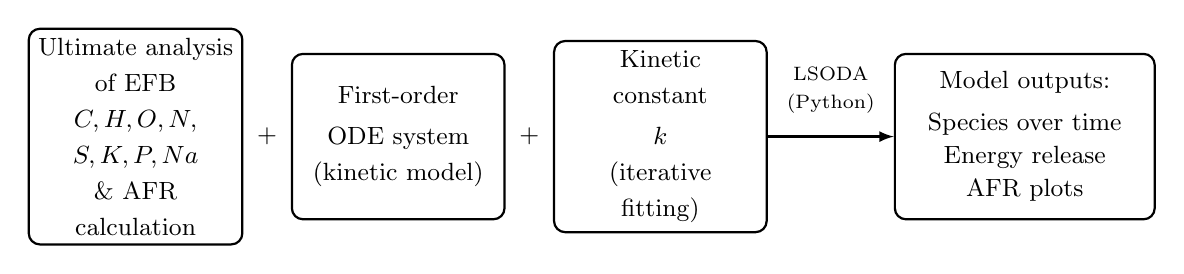
\begin{tikzpicture}[
    font=\small,
    >=latex,
    node distance=0.6cm,
    block/.style={
        draw,
        thick,
        rounded corners,
        align=center,
        minimum width=2.7cm,
        minimum height=2.1cm
    }
]

% Bloques principales
\node[block] (fuel) {%
    Ultimate analysis \\[2pt]
    of EFB \\[2pt]
    \textit{$C,H,O,N,$} \\[2pt]
    \textit{$S,K,P,Na$} \\[2pt]
    \& AFR \\[2pt]
    calculation
};

\node[right=0.05cm of fuel] (plus1) {$+$};

\node[block, right=0.05cm of plus1] (ode) {%
    First-order \\[4pt]
    ODE system \\[2pt]
    (kinetic model)
};

\node[right=0.05cm of ode] (plus2) {$+$};

\node[block, right=0.05cm of plus2] (params) {%
    Kinetic \\ [2pt]
    constant \\[4pt]
    $k$ \\[2pt]
    (iterative \\[2pt]
    fitting)
};

% Bloque de salidas con más separación
\node[block, right=1.6cm of params, minimum width=3.3cm, minimum height=2.1cm] (outputs) {%
    Model outputs: \\[4pt]
    Species over time \\[1pt]
    Energy release \\[1pt]
    AFR plots
};

% Flecha y texto LSODA
\path (params.east) -- (outputs.west) coordinate[midway] (mid);
\draw[->, thick] (params.east) -- (outputs.west);

\node[above=5pt of mid, align=center] {%
    \scriptsize LSODA \\[-1pt]
    \scriptsize (Python)
};

\end{tikzpicture}%
}
\caption{General schematic of the computational workflow for the combustion model.}
\label{fig:workflow}
\end{figure}



\subsection{Mass Balance}

A mass balance is the core of chemical reaction modeling that ensures the conservation of matter during physical and chemical transformations. In combustion systems, it allows tracking how the initial mass of fuel components is progressively converted into combustion products. This provides a basis for quantifying the evolution of each species over time.\\

To simulate this process in a realistic and predictive way, the mass balance is a system of first-order Ordinary Differential Equations (ODE), where each equation represents the rate of change of a chemical species. These equations are governed by kinetic rate expressions of the Arrhenius type, which relate reaction rates to temperature and activation energy. Together, these elements form a single, integrated modeling approach that captures both the chemical dynamics and the temporal evolution of species during biomass combustion.



\subsubsection{Elemental compositions of EFB and PMF}
\label{Initial Conditions for EFB and PMF Combustion}\\

%The computational model simulates the chemical evolution of the system over time through the set of first-order differential equations for the species.
%The set of first-order ODE for the species are governed by the initial molar concentrations. 
%Therefore, initial conditions require the chemical characterization of the EFB and PMF and their specific elemental compositions.\\

\begin{comment}
The initial concentration of species are calculated on a biomass boiler basis, such as specific capacity, operational temperature, allowable pressure and combustion chamber size as related on table \ref{tab:boiler_specs}.\\

\begin{table}[H]
\centering
\caption{General specifications of the biomass boiler.}
\label{tab:boiler_specs}
\begin{tabular}{ll}
\hline
\textbf{Parameter} & \textbf{Value} \\
\hline
Capacity & 30~t/h \\
Operational Temperature & 573.15~K \\
Allowable Pressure & 10--30~bar \\
Combustion Chamber Size & 360~m$^3$ \\
\hline
\end{tabular}
\end{table}

The base mass used for both fuels was 8.33 kg/s, equivalent to a 30 t/h feeding rate in medium-sized biomass boilers. These specifications serve as conditions of a biomass boiler to constrain the kinetic model and ensure that the EFB and PMF quantities, its molar concentrations of elements equivalent on the rate and initial temperature correspond to a realistic scenario.\\
\end{comment}

%To translate this feeding rate into initial species concentrations, it is first necessary to characterize the elemental composition of each fuel.
%The elemental composition of each fuel is the departing step for the calculation of initial species concentrations. 
The set of first-order ODE for the species are governed by the initial molar concentrations. Elemental composition data for EFB and PMF are collected from a literature review and reported on a dry basis. PMF composition has been obtained as part of the comparative analysis in \cite{Idris2012}, and presented here in Table~\ref{tabla:compPalmiste}. For EFB, composition values have been extracted from seven scientific studies and averaged to yield representative results, see Table \ref{tab:composition2_transposed}.\\ 

\begin{table}[H]
\begin{center}
\caption{Elemental composition of PMF reported by \cite{Idris2012} on a dry basis \%}
\label{tabla:compPalmiste}
\begin{tabular*}{6cm}{l p{3cm}} \hline
\textbf{Element} & \textbf{Percentage of mass(\%)} \\ \hline
Carbon (C) & 51.52 \\
Hydrogen (H) & 5.45 \\
Oxygen (O) & 40.91 \\
Nitrogen (N) & 1.89 \\
Sulfur (S) & 0.23 \\ \hline
\end{tabular*}
\end{center}
\end{table}


\begin{table}[H]
\centering
\caption{Elemental composition of EFB reported by different authors on a dry basis \%}
\label{tab:composition2_transposed}
\renewcommand{\arraystretch}{1.2}
\small
\begin{tabularx}{\textwidth}{lcccccccc}
\hline
\textbf{Author} & \textbf{C} & \textbf{H} & \textbf{O} & \textbf{N} & \textbf{S} & \textbf{K} & \textbf{P} & \textbf{Na} \\
\hline
Olisa \& Kotingo \cite{Olisa2014}         & 43.8  & 6.2   & 42.65 & 0.44 & 0.09  & --   & --     & --    \\
García-Núñez et al. \cite{GarciaNunez2006} & 40.88 & --    & --    & 0.87 & 0.09  & 2.23 & 0.057  & 0.01 \\
Ninduangdee et al. \cite{Ninduangdee2015}  & 48.2  & 6.49  & 31.74 & 0.47 & 0.10  & --   & --     & --    \\
Madhiyanon et al. \cite{Madhiyanon2012}    & 40.7  & 5.4   & 47.0  & 0.3  & 1.1   & --   & --     & --    \\
Ramírez et al. \cite{Ramirez2011}          & 42.8  & 6.4   & 35.8  & 0.8  & 0.1   & --   & --     & --    \\
Kaniapan et al. \cite{Kaniapan2021}        & 42.8  & 6.2   & 50.44 & 0.47 & 0.09  & --   & --     & --    \\
Bayona-Roa et al. \cite{BayonaRaquis}      & 48.03 & 6.47  & 39.65 & 0.77 & 0.084 & --   & --     & --    \\
\hline
\end{tabularx}
\end{table}

For each specie (C, H, O, N, S, potassium (K), phosphorus (P), sodium (Na)), the number of moles is calculated by dividing the mass obtained from the respective mass fractions by the atomic molar mass,

\begin{equation}
\label{mol}
n_i = \frac{m_i}{MW_i},
\end{equation}
where $n_i$ is the molar concentration, $m_i$ is the fraction mass, and $MW_i$ is the atomic mass weight of each $i-$th species. Moreover, to express the initial conditions in terms of volumetric concentrations (mol/m$^3$), the number of moles of each element is divided by the active combustion volume,
\begin{equation}
\label{volumetricX}
C_{i,0} = \frac{n_i}{V_{\text{chamber}}},
\end{equation}
where the initial volumetric concentrations ($C_{i,0}$) are then used as the initial input for solving the system of ordinary differential equations.

\subsubsection{Kinetic Modelling of Combustion}\\
\label{Kinetic Modelling of Comustion}

%Understanding how chemical reactions evolve during combustion predicts the concentration and generation of the products. 
Kinetic chemical modeling describes the reaction rates that govern the transformation of fuel and oxidizer into combustion products. Rather than relying on overall balances, this approach focuses on the dynamics of each chemical species involved. 
The consumption and generation of chemical species is modeled via a first-order ODE arising from the mass balance. This mathematical models express the time change of the species concentration as a function of its interaction with other species:
\begin{equation}
    \frac{dX_i}{dt} = - f_i (k_1 X_1,k_2X_2,\ldots,k_iX_i,\ldots,k_jX_j),
\end{equation}
where $X_i$ is the molar concentration, $k_i$ is a kinetic coefficient, and $f_i$ is a function describing the interaction of the $i$-th species with another $j-$th species.\\

Variables $X_i$ represent any chemical species (e.g., C, H, O$_2$), while the kinetic terms capture reactivity rates and constraints imposed by the comburent. The differential model becomes a powerful tool for representing non-linear interactions and feedback mechanisms that characterize the combustion of complex fuels such as biomass. The formulation therefore applies to dry biomass combustion, where multiple elemental reactions occur simultaneously and at different rates, depending on temperature and chemical environment.\\

This formulation is applied separately to both EFB and PMF, allowing for the characterization of each fuels specific kinetic behavior based on their unique elemental compositions and reactivity profiles. This dual application enables comparative analysis and model adaptability to varying biomass types. The resulting structure supports the representation of complex reaction networks while remaining tractable through lumped kinetic terms.\\

The proposed model for PMF tracks 10 species, including 5 main reactants  (C, H, N, S, O$_2$) and 5 products (carbon dioxide (CO$_2$), water vapor (H$_2$O), sulfur dioxide (SO$_2$), nitrogen gas (N$^{\text{out}}$), nitrogen oxides (NO$_x$)). In the case of EFB, the model tracks 15 species, including 8 main reactants (C, H, N, S, K, P, Na, O$_2$) and 7 products (CO$_2$, H$_2$O, SO$_2$, N$^{\text{out}}$, potassium oxide (K$_2$O), phosphorus pentoxide (P$_2$O$_5$), sodium oxide (Na$_2$O)). See tables \ref{tab:Equations_PMF} and \ref{tab:Equations_EFB} for the detail formulation of each kinetic model for PMF and EFB, respectively. \\

\begin{table}[H]
\centering
\caption{Combustion kinetics equations for PMF}
\label{tab:Equations_PMF}
\renewcommand{\arraystretch}{1.3}
\small

\begin{tabularx}{\textwidth}{l >{\centering\arraybackslash}X c c}
\hline
\textbf{Species} &
\textbf{Equation} &
\makecell[c]{\textbf{Constant $k$}\\[2pt] [m$^3$/mol\cdot  s]} &
\makecell[c]{\textbf{Initial concentration}\\[2pt] $C_{i,0}$ [mol/m$^3$]} \\[4pt]
\hline

C & 
$\displaystyle \frac{dC}{dt} = -k_C \frac{C\,O_2}{N}$ &
$1.07 \times 10^{-5}$ & 
2.8383 \\[4pt]

H & 
$\displaystyle \frac{dH}{dt} = -k_H \frac{H\,O_2}{N}$ &
$6.42 \times 10^{-7}$ & 
3.6030 \\[4pt]

N &
$\displaystyle \frac{dN}{dt} = -k_N \frac{N_i\,O_2}{N}$ &
$1.71 \times 10^{-7}$ & 
0.0892 \\[4pt]

S &
$\displaystyle \frac{dS}{dt} = -k_S \frac{S\,O_2}{N}$ &
$2.14 \times 10^{-7}$ & 
0.0047 \\[4pt]

N$_2$ & 
$\displaystyle \frac{dN_2}{dt} = 0$ &
-- & 
4.2250 \\[4pt]

O$_2$ & 
\makecell[c]{
$\displaystyle \frac{dO_2}{dt} = -\left(k_C X_C + k_H X_H$ \\[2pt]
$\displaystyle + k_N X_{N_i} + k_S X_S\right) \frac{O_2}{N}$
} &
$k_O(t,k_i,X_i)$ & 
3.7423 \\[4pt]

CO$_2$ & 
$\displaystyle \frac{dCO_2}{dt} = k_C \frac{C\,O_2}{N}$ & 
$1.07 \times 10^{-5}$ & 
0 \\[4pt]

H$_2$O & 
$\displaystyle \frac{dH_2O}{dt} = k_H \frac{H\,O_2}{N}$ &
$6.42 \times 10^{-7}$ & 
0 \\[4pt]

SO$_2$ &
$\displaystyle \frac{dSO_2}{dt} = k_S \frac{S\,O_2}{N}$ &
$2.14 \times 10^{-7}$ & 
0 \\[4pt]

NO$_x$ &
$\displaystyle \frac{dNO_x}{dt} = \frac{N\,O_2}{N}$ &
-- & 
0 \\[6pt]  % Espacio arriba de la línea final
\hline
\end{tabularx}
\end{table}


\begin{table}[H]
\centering
\caption{Combustion kinetics equations for EFB}
\label{tab:Equations_EFB}
\renewcommand{\arraystretch}{1.3}
\small

\begin{tabularx}{\textwidth}{l >{\centering\arraybackslash}X c c}
\hline
\textbf{Species} &
\textbf{Equation} &
\makecell[c]{\textbf{Constant $k$}\\[2pt] [m$^3$/mol\cdot  s]} &
\makecell[c]{\textbf{Initial concentration}\\[2pt] $C_{i,0}$ [mol/m$^3$]} \\[4pt]
\hline


C & 
$\displaystyle \frac{dC}{dt} = -k_C \frac{C\,O_2}{N}$ &
$1.07 \times 10^{-7}$ & 
2.4180 \\[4pt]

H & 
$\displaystyle \frac{dH}{dt} = -k_H \frac{H\,O_2}{N}$ &
$6.42 \times 10^{-7}$ & 
4.0922 \\[4pt]

N &
$\displaystyle \frac{dN}{dt} = -k_N \frac{N_i\,O_2}{N}$ &
$1.71 \times 10^{-7}$ & 
0.0278 \\[4pt]

S &
$\displaystyle \frac{dS}{dt} = -k_S \frac{S\,O_2}{N}$ &
$2.14 \times 10^{-7}$ & 
0.0049 \\[4pt]

K & 
$\displaystyle \frac{dK}{dt} = -k_K \frac{K}{N}$ &
$2.14 \times 10^{-7}$ & 
0.0378 \\[4pt]

P &
$\displaystyle \frac{dP}{dt} = -k_P \frac{P}{N}$ &
$1.71 \times 10^{-7}$ & 
0.0012 \\[4pt]

Na &
$\displaystyle \frac{dNa}{dt} = -k_{Na} \frac{Na}{N}$ &
$1.71 \times 10^{-7}$ & 
0.0003 \\[4pt]

N$_2$ & 
$\displaystyle \frac{dN_2}{dt} = 0$ &
-- & 
3.8888 \\[4pt]

O$_2$ & 
\makecell[c]{
$\displaystyle \frac{dO_2}{dt} = -\left(k_C X_C + k_H X_H$ \\[2pt]
$\displaystyle + k_N X_{N_i} + k_S X_S + k_K X_K$ \\[2pt]
$\displaystyle + k_P X_P + k_{Na} X_{Na}) \right) \frac{O_2}{N}$
} &
$k_O(t,k_i, X_i)$ & 
5.1474 \\[4pt]

CO$_2$ & 
$\displaystyle \frac{dCO_2}{dt} = k_C \frac{C\,O_2}{N}$ &
$1.07 \times 10^{-7}$ & 
0 \\[4pt]

H$_2$O &
$\displaystyle \frac{dH_2O}{dt} = k_H \frac{H\,O_2}{N}$ &
$6.42 \times 10^{-7}$ & 
0 \\[4pt]

SO$_2$ &
$\displaystyle \frac{dSO_2}{dt} = k_S \frac{S\,O_2}{N}$ &
$2.14 \times 10^{-7}$ & 
0 \\[4pt]

K$_2$O & 
$\displaystyle \frac{dK_2O}{dt} = k_K \frac{K}{N}$ &
$2.14 \times 10^{-7}$ & 
0 \\[4pt]

P$_2$O$_5$ & 
$\displaystyle \frac{dP_2O_5}{dt} = k_P \frac{P}{N}$ &
$1.71 \times 10^{-7}$ & 
0 \\[4pt]

Na$_2$O & 
$\displaystyle \frac{dNa_2O}{dt} = k_{Na} \frac{Na}{N}$ &
$1.71 \times 10^{-7}$ & 
0 \\[6pt]
\hline
\end{tabularx}
\end{table}


Although the initial formulation of our model included temperature-dependent kinetic rate constants $k_i$ based on the Arrhenius expression, this variation proved to have negligible influence on the resulting energy output due to the narrow temperature range defined in the simulation. Therefore, a simplified approach is adopted in which constant $k$ values are assigned to each species from NIST chemical database \cite{NISTkinetics}.  These constants have been calibrated to reproduce the expected combustion behavior, following a common practice in semi-empirical models of biomass combustion \cite{GarciaNunez2006}, as explained explained at section \ref{energy_section}.  This calibration-based method ensures computational efficiency while maintaining physical relevance within the operating range considered. Nevertheless, since the model assumes no temperature dependency, this constitutes a limitation with respect to representing real combustion behavior, as temperature fluctuations can alter reaction rates and modify the gradients of species concentrations at specific time intervals. Even so, using constant kinetic coefficients provides a stable description of the overall reaction progress, avoiding numerical oscillations that may arise from strong temperature–rate coupling. Importantly, this simplification does not affect the final concentrations obtained at the end of the process. \\

The empirically selected constants are also presented in tables \ref{tab:Equations_PMF} and \ref{tab:Equations_EFB} for PMF and EFB, respectively. To ensure complete oxygen consumption in each reaction, the $k$ constant for this species changes over time. Thus, it is defined for the initial instant as $k_O$ in tables \ref{tab:Equations_PMF} and \ref{tab:Equations_EFB}.  \\ 

%CITAAAAAAAAAAAAAAAAAAAA (Determination of Kinetic Parameters of Thermal Degradation of Palm Oil Mill by Products Using Thermogravimetric Analysis and Differential Scanning Calorimetry)


\subsubsection{Stoichiometry}
\label{Calculus of the required Oxygen for combustion}\\

To estimate the amount of oxygen needed for complete combustion of the biomass fuels (EFB and PMF), a stoichiometric analysis is performed based on their elemental compositions. The process focuses on the primary combustible elements (C, H, and S), which contribute directly to the energy released. The exclusion of certain elements from this calculation is justified by the varying magnitudes of the kinetic reaction constants between each element and oxygen, as discussed in Section~\ref{Kinetic Modelling of Comustion}. Furthermore, it is assumed that atmospheric air is composed of approximately 21\% O$_2$ and 79\% N$_2$, corresponding to a molar ratio of 1:3.76 for O$_2$ to N$_2$, which is employed to estimate the total mass of air required for combustion.\\


The stoichiometric balances give for PMF: 

\begin{multline}
    \quad C_{595}H_{750}O_{355}N_{19}S \rightarrow 
    595CO_2 + 375H_2O + 19NO_2 + SO_2 + 2350N_2,
\end{multline}

and for EFB:

\begin{multline}
    \quad C_{488}H_{821}O_{344}N_6S + 0.49K + 0.056P + 0.024Na \rightarrow 488CO_2 + 410.5H_2O\\ + SO_2 + 1971.47N_2 + 0.245K_2O + 0.028P_2O_5 + 0.012Na_2O.
\end{multline}


\subsubsection{Estimation of AFR}\\
\label{AFREST}
The stoichiometric AFR is calculated using the following expression:

\begin{equation}
    \text{AFR} = \frac{m_{\text{air}}}{m_{\text{fuel}}}.
\end{equation}

The AFR is a key parameter to evaluate the combustion behavior of different biomass types, as it reflects the theoretical mass of air required per unit mass of fuel (as in the stoichiometric balances, for instance). Differences in AFR between EFB and PMF arise from variations in their elemental composition, particularly the relative proportions of C, H and S. These differences are quantitatively assessed in the section~\ref{results}.

\subsection{Combustion Energy Estimation} 
\label{energy_section}

The estimation of the energy released during biomass combustion is essential for evaluating fuel performance and thermal designing. In this study, both a thermodynamic approach and empirical calibration are used to characterize the energy output of EFB and PMF combustion.\\

To estimate the heat released during combustion from a thermodynamic standpoint, the standard enthalpy of formation ($\Delta H_f^\circ$) is used. This quantity reflects the heat change when a compound is formed from its elemental constituents at standard conditions (298 K, 1 atm). The net enthalpy change of the reaction is calculated as:

\begin{equation}
    \Delta H_{\rm rxn}(t) = \sum n_{r,i}(t) \Delta H_{f,i}^{\circ}(\text{reactants}) - \sum n_{p,i}(t) \Delta H_{f,i}^{\circ}(\text{products}),
\end{equation}

where $\Delta H_{\rm rxn}(t)$ is the reaction (combustion) enthalpy in kJ/mol, $\Delta H_f^\circ$ is the standard enthalpy of formation of species $i$, and $n_{r,i}(t)$ and $n_{p,i}(t)$ are the molar concentrations of reactants and products, respectively, arising from the mass balance solution at each time instant.\\

This formulation neglects the inherent moisture content of the biomass, isolating the chemical energy contribution of the fuel, excluding the endothermic effects associated with water evaporation during combustion. Section~\ref{Moisture Content} presents valuable insights for this assumption.\\

Once the energy release is estimated, the temperature of the adiabatic flame is calculated, assuming no heat losses to the environment. This temperature is derived from the energy released during combustion, under the assumption that all the energy goes into heating the combustion products. The change in temperature $(\Delta T (t))$ is calculated using the following equation:

\begin{equation}
\Delta T = \frac{\Delta H_{\rm rxn}(t)}{\sum_i m_i c_{p,i}},
\end{equation}

where $c_{p,i}$ is the specific heat capacity at constant pressure of each $i-$th species. Therefore the overall heat capacity is calculated as a weighted average based on the concentrations of the different species present in the biomass. This provides the temperature of the combustion products without considering any heat losses to the surroundings.\\


The corresponding power output is computed as the time derivative of the combustion enthalpy:
\begin{equation}
\text{Power}(t) = \frac{d\Delta H_{\rm rxn}(t)}{dt}.
\end{equation}

The energy released during the combustion process is estimated using the following methodology: the molar quantities of each species are dynamically obtained from the kinetic simulation presented in previous sections, while the standard enthalpies of formation are obtained from thermochemical reference tables \cite{AtkinsPChem}. The main values used in this study are summarized in Table~\ref{tabla:entalpias_formacion}:\\

\begin{table}[H]
\begin{center}
\caption{Standard enthalpy of formation for selected combustion products \cite{AtkinsPChem}.}
\label{tabla:entalpias_formacion}
\begin{tabular*}{6cm}{l p{3cm}} \hline
\textbf{Compound} & $\boldsymbol{\Delta H_f^\circ}$ \textbf{[kJ/mol]} \\ \hline
CO$_2$           & $-393.5$ \\
H$_2$O           & $-241.82$ \\
SO$_2$           & $-296.83$ \\
NO$_x$           & $33.2$ \\
K$_2$O           & $-363.2$ \\
P$_2$O$_5$       & $-1340$ \\
Na$_2$O          & $-414$ \\ \hline
\end{tabular*}
\end{center}
\end{table}

Zero enthalpies of formation are assumed for the chemical elements:
\begin{center}
$\Delta H_f^{\circ}(\text{C}, \text{H}, \text{O}_2, \text{N}, \text{S}, \text{K}, \text{P}, \text{Na}) = 0$
\end{center}

Reference LHV values from literature are used for both EFB and PMF to estimate the theoretical energy that a given mass of biomass could release. And using this energy target as a benchmark, an iterative fitting procedure is implemented to determine appropriate reaction rate constants for each fuel with the objective of obtaining simulation results that closely matched the expected energy release for the combustion of the biomass. This iterative procedure is governed by systematic adjustments to the kinetic constants: increasing a constant accelerates the corresponding reaction rate, whereas decreasing it slows the consumption of the associated species. After each adjustment, the cumulative energy released is recalculated and compared against the theoretical LHV-based target. Throughout this process, the relative magnitudes among the constants are preserved to maintain physically coherent reactivity—for instance, ensuring that hydrogen oxidation proceeds faster than carbon oxidation. This strategy allows the global heat release to converge toward the theoretical value while retaining realistic reaction behavior.\\





This parameter-fitting strategy enables the selection of a suitable set of kinetic constants that capture the energy performance of both fuels under similar boiler conditions, and once validated, these constants are used in all subsequent simulations and sensitivity analyses.\\

\subsection{Numerical Solution}\\

The complete systems of ODEs in tables \ref{tab:Equations_PMF} and \ref{tab:Equations_EFB} are solved using Python function \textbf{scipy.\-integrate.\-odeint}
 over a simulation time of 3,000 milliseconds and 6,000 time steps. The solution provides temporal profiles for each species, allowing for the analysis of combustion dynamics, depletion of reactants, and formation of key products. These results are further used in the subsequent energy evaluations.\\

The \texttt{odeint} function in Spicy Python Library implements the LSODA algorithm, which dynamically alternates between the non-stiff Adams--Bashforth--Moulton method and the stiff Backward Differentiation Formula (BDF) \cite{HindmarshODEPACK}, depending on the behavior of the system. This adaptive strategy ensures numerical stability and computational efficiency without the need for manual tuning. In this case, the system is not explicitly stiff, but involves strongly coupled species and moderately fast reaction rates, for which LSODA can switch between methods as needed.\\

To obtain valid concentration profiles, several iterations of the kinetic model are performed for both EFB and PMF. The kinetic constants are fine-tuned to ensure complete carbon burnout while achieving total energy release values consistent with theoretical yields derived from the LHV and the inlet biomass mass. The model is executed repeatedly with adjusted parameters until the heat release curves closely matched the expected thermal profiles for both fuels. This dual-level validation (mass conservation and energy release) ensures that the model faithfully captures the essential dynamics of biomass combustion. Each simulation cycle required only 10 to 15 physical seconds, which greatly facilitated parameter refinement.\\

Once the species and energy outputs align with the expected theoretical values, extra simulations are performed with different initial air concentrations to evaluate the effect of AFR on combustion performance. For each case, the energy released per unit mass and its temporal profile are analyzed. This allows the identification of AFR values that maximizes thermal efficiency for each fuel type. The ability to modify inputs and re-run scenarios efficiently made it possible to assess AFR sensitivity without compromising the consistency of the combustion model.\\

All simulations, data processing, and visualizations were implemented entirely in Python, allowing for flexible manipulation of model parameters and fast execution cycles throughout the entire analysis.

% ------------------- RESULTS ----------------------
\section{Results and discussion}
\label{results}
% VALIDATION OF THE MODEL
\subsection{Validation of the model}
\label{Validation of the model}\\

%For every simulation, the total chamber volume is considered as 360~m$^3$, but only 35\% of this (i.e., 126~m$^3$) is the effective reaction zone. Therefore, $V_{\text{chamber}}=$126~m$^3$.\\

Model validation is established through three key criteria: the complete conversion of C to CO$_2$, which ensures the absence of unburned species and eliminates the need for additional air inlets, and the consistency between the energy released by the model and the theoretical energy yield ($E_{\text{t}}$) of each biomass; and third the numerical convergence of the differential system based on the evolution of species-specific residuals. \\

The latter criterion is assessed through a residual analysis that traces the discrete error propagation of each species over time, establishing a convergence threshold of $1\times10^{-4}$, equivalent to a relative error below 0.01\%. This threshold is allways reached before 3000~ms, after which all residuals continued to decrease and stabilized at values significantly below the convergence limit (on the order of $10^{-8}$–$10^{-10}$), indicating a minimal propagation of numerical error and confirming the model’s strong temporal stability. Within this 3000~ms period, most of reactive species (particularly carbon) are completely consumed, consistent with the defined non-continuous fuel injection condition. Extending the simulation beyond this point would not alter the results, as the concentrations had already stabilized.\\

Due to the lack of studies reporting time-resolved species evolution for EFB and PMF, the validation threshold is defined based on the variation in LHV reported in the literature, as presented in Table \ref{tab:tableLHV}.\\

\begin{table}[H]
\begin{center}
\caption{Experimental LHV of EFB and PMF reported by different authors}
\label{tab:tableLHV}
\renewcommand{\arraystretch}{1.2}
\begin{tabular*}{\linewidth}{@{\extracolsep{\fill}} l l l} 
\hline
\textbf{Author} & \textbf{EFB} [MJ/kg] & \textbf{PMF} [MJ/kg] \\ 
\hline
Ninduangdee et al. (2015) \cite{Ninduangdee2015} & 18.9 & -- \\
Olisa y Kotingo (2014) \cite{Olisa2014}       & 19.25 & -- \\

Bayona-Roa et al. (2023) \cite{BayonaRaquis}      & 16.27 & -- \\

Idris et al. (2012) \cite{Idris2012}     & 16.8 & 19 \\
\hline
\textbf{Average} & \textbf{17.66} & \textbf{19} \\

\hline
\end{tabular*}
\end{center}
\end{table}

%The average LHV value from table \ref{tab:tableLHV} is: $\text{LHV}_{\rm EFB} = 17.66 \, \text{MJ/kg}$ \cite{BayonaRaquis} and $\text{LHV}_{\rm PMF} = 19 \, \text{MJ/kg}$ \cite{Idris2012}.

%These values represent the theoretical energy content available per unit mass of biomass under ideal combustion conditions and serve as reference targets in the modeling process. \\

Using the average LHV of 17.66 MJ/kg for the EFB as a reference, the difference with respect to the highest reported LHV for EFB in Table \ref{tab:tableLHV} (19.25 MJ/kg) is 8.62\%. Similarly, the difference with the lowest experimentally measured reported value (16.27 MJ/kg) is 7.87\%. These margins reflect the inherent experimental variability in LHV determinations. \\

%Since the total energy released during combustion is directly proportional to the LHV of the fuel and the mass burned, variations in the reported LHV values directly translate into expected variations in energy release. For this reason, the range defined by this link provides a rational basis for establishing an acceptance threshold.\\

Accordingly, a deviation of up to 8.62\% is accepted, as it represents the highest variation among the referenced LHV values. This criterion accounts for the absence of species-resolved experimental data for EFB and PMF combustion, while still enabling a robust evaluation of the model predictive accuracy. Based on this approach, the model is considered validated when the predicted energy yield falls within this tolerance, demonstrating consistency with experimentally-derived LHV values. \\

Finally, the simulation is limited to 3000~ms, since by that time all convergence criteria are satisfied and the residuals stabilize below the established threshold. This time window is also defined based on the physical behavior of the system, which corresponds to a single-injection process rather than a continuous-feed configuration. In the absence of experimentally-defined reaction times for the EFB and PMF biomass, the evolution of the residuals and the complete depletion of reactants are used as indicators to define the simulation endpoint. Beyond this point, the variables exhibit no further changes, confirming that both the numerical and physicochemical conditions of the combustion process stabilizes.

\subsubsection{PMF model validation}


The theoretical energy yield corresponding to PMF is obtained by multiplying its LHV by the total mass of biomass input used in the simulation:

\[
E_{\text{t}} = \text{LHV}_{\text{PMF}} \times m_{\text{PMF}} = 19\ \text{MJ/kg} \times 8.33\ \text{kg} = 158.27\ \text{MJ}
\]

The numerical model reports an energy output of approximately $150\ \text{MJ}$ (see Figure~\ref{fig:PalmisteEnergy}), then the relative error between the simulated and theoretical values is 5.51\%. This resulting error satisfy the acceptance range established, which reinforces the reliability of the model in accurately capturing the combustion behavior of PMF. Therefore, kinetic equations, initial concentrations and constants in table \ref{tab:Equations_PMF} are validated.\\

\subsubsection{EFB model validation}
\label{efbmodelval}
A similar comparison is carried out for EFB. The numerical energy yield is calculated using the LHV of EFB and the corresponding biomass mass:

\[
E_{\text{t}} = \text{LHV}_{\text{EFB}} \times m_{\text{EFB}} = 17.66\ \text{MJ/kg} \times 8.33\ \text{kg} = 147.11\ \text{MJ}
\]

The numerical model output for EFB shows a total energy release of approximately 140  
 $\text{MJ}$ (see Figure~\ref{fig:EFBEnergy}), thus the relative error is 5.07\%. As in the case of PMF, the error meets the condition of the acceptance value, confirming that the model accurately reproduces the expected energy behavior of EFB under combustion conditions. Consequently, table \ref{tab:Equations_EFB} presents the validated kinetic equations, initial concentrations and constants.\\

 \subsubsection{Model validation insights}

The validation of the present kinetic model relies exclusively on the energy–output consistency. This, by adopting the theoretical LHV as the reference value. The LVH-error approach is necessary because currently no calorimetric measurements are available for reaction times or heat release of EFB combustion under controlled laboratory conditions. Consequently, a rigorous sensitivity analysis of the kinetic parameters (such as a systematic variation of the reaction constants and a quantitative minimization of the LHV error) can not be performed.\\

It is also important to highlight that no reaction–rate parameters have been reported in the scientific literature for EFB and PMF combustion. Therefore, the present model provides only an initial kinetic approximation that ensures mass conservation and correct energy release, 
but it cannot yet be calibrated against experimental curves of species evolution or heat–release rates. This limitation prevents the formulation of an error–propagation analysis, as the uncertainties associated with the kinetic constants are not known.\\

Future research should include TGA and DTGA experiments under controlled experimental combustion tests to determine real heat–release profiles, reaction times, and species–conversion rates for EFB and PMF. These measurements will enable the identification of optimal kinetic constants and the implementation of a formal sensitivity analysis. Once such experimental 
data becomes available, the present model can be refined to provide high–fidelity kinetic parameters for EFB combustion, strengthening its predictive capacity for integration into CFD frameworks and boiler–design studies.\\

%These results validate the developed model as capable of achieving a combustion analysis. It is capable of reproducing the kinetic behavior of different biomass fuels, making it suitable for a wide range of investigative and analytical applications.

\subsection{Simulation results}\label{simresults}

% ******** PALMISTE GRAFICAS ******

\subsubsection{Temporal evolution of chemical species during PMF combustion}

Figure~\ref{fig:PalmisteConcentraciones} shows the temporal evolution of the main chemical species during the combustion of PMF.

\begin{figure}[H]
    \centering
    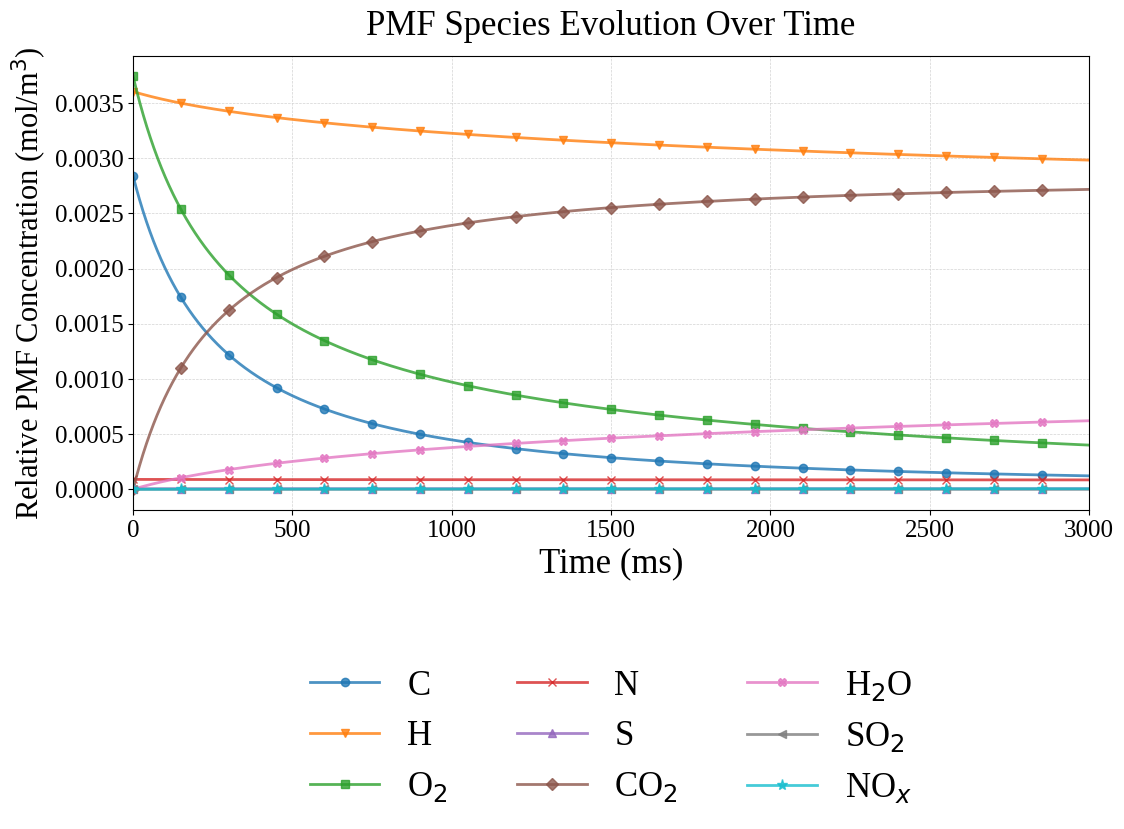
\includegraphics[width=1\textwidth]{FIGURES/respmfcombustiontimes9.png}
    \caption{Species concentration profiles during PMF combustion.}
    \label{fig:PalmisteConcentraciones}
\end{figure}



At the initial stage of the reaction (1,000 ms), the concentrations of C and O$_2$ decrease similarly over 60\% of their initial concentration, meanwhile H curve reduces to 0.0005. This is indicative of the rapid oxidation that occurs during the initial phase of combustion. By millisecond 1,500, the conversion of C into CO$_2$ and H into H$_2$O occurs, with both products reaching steady-state 0.0027 and 0.001 concentrations respectively, as the reactants are consumed.
\\

N$_2$ concentration remains constant at approximately 0.0005 throughout the process. The formation of NO$_x$ and SO$_2$ is minimal, both staying below 0.0001, indicating limited conversion of fuel-bound nitrogen and sulfur. The trends suggest that NO$_x$ emissions are sensitive to combustion conditions, particularly temperature.
\\

Most concentration changes occur within the first 2,000 milliseconds of the simulation. After this point, species other than C, H, and H$_2$O maintain stable values. C is almost entirely converted to CO$_2$ by the end of the simulation, indicating that the kinetic constants reported in section \ref{Kinetic Modelling of Comustion} result in complete C burnout, thus avoiding the formation of unburned residues.\\

\subsubsection{Energy release and power output during PMF combustion}
\label{Energy release and instantaneous power output during PMF combustion}\\

\begin{figure}[H]
    \centering
    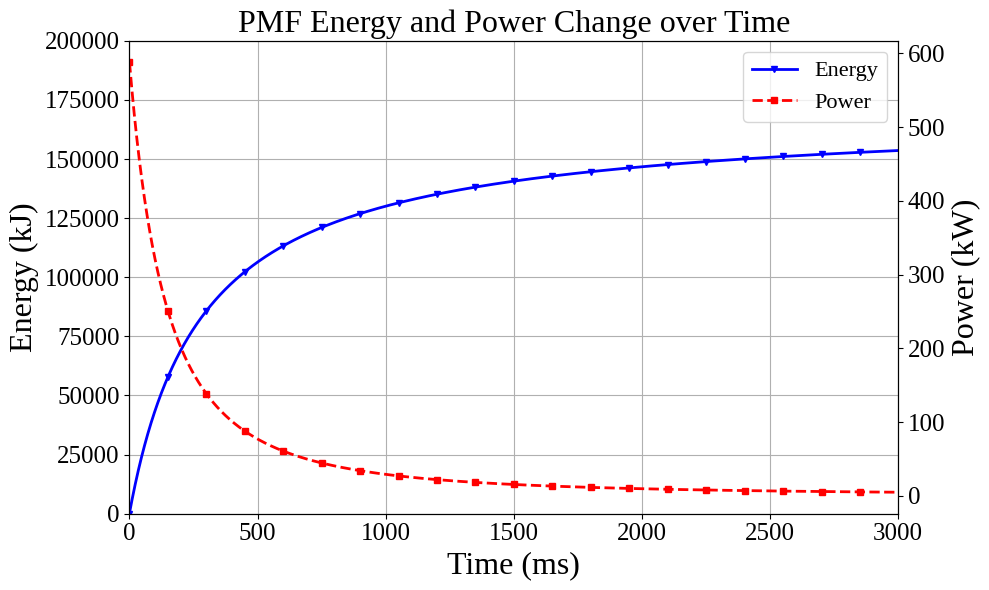
\includegraphics[width=\columnwidth]{FIGURES/respmfenergytimes6.png}
    \caption{Temporal evolution of cumulative combustion energy and power output for PMF. The solid curve shows the cumulative energy released (kJ) as combustion progresses, while the dashed curve represents the instantaneous power output, obtained as the time derivative of the energy curve.}
    \label{fig:PalmisteEnergy}
\end{figure}


Figure~\ref{fig:PalmisteEnergy} shows the energy dynamics of PMF combustion. Approximately 120,000~kJ (80\%) of the total combustion energy is released within the first 1,000 ms. After this point, the energy increase slows, with the curve approaching an asymptote near 155,000~kJ.  Finally, the total energy released converges toward a maximum of approximately 150,000~kJ (150~MJ), consistent with complete oxidation of the fuel mass defined in the simulation and the LHV of the biomass: 19~MJ/kg \cite{Idris2012}.\\


Similarly, the evolution of combustion power begins with a sharp power peak close to 600~kW, driven by rapid ignition and volatile release. This is followed by a pronounced exponential decay, as fuel availability declines and combustion transitions into a diffusion-controlled regime. By approximately 400~ms, the power output falls below 100~kW, indicating that most of the heat is released in the early stages of the reaction.\\


\subsubsection{Effect of AFR on heat release and adiabatic temperature during PMF combustion}\\
\label{Heat release variation with AFR during PMF combustion}

\begin{figure}[H]
    \centering
    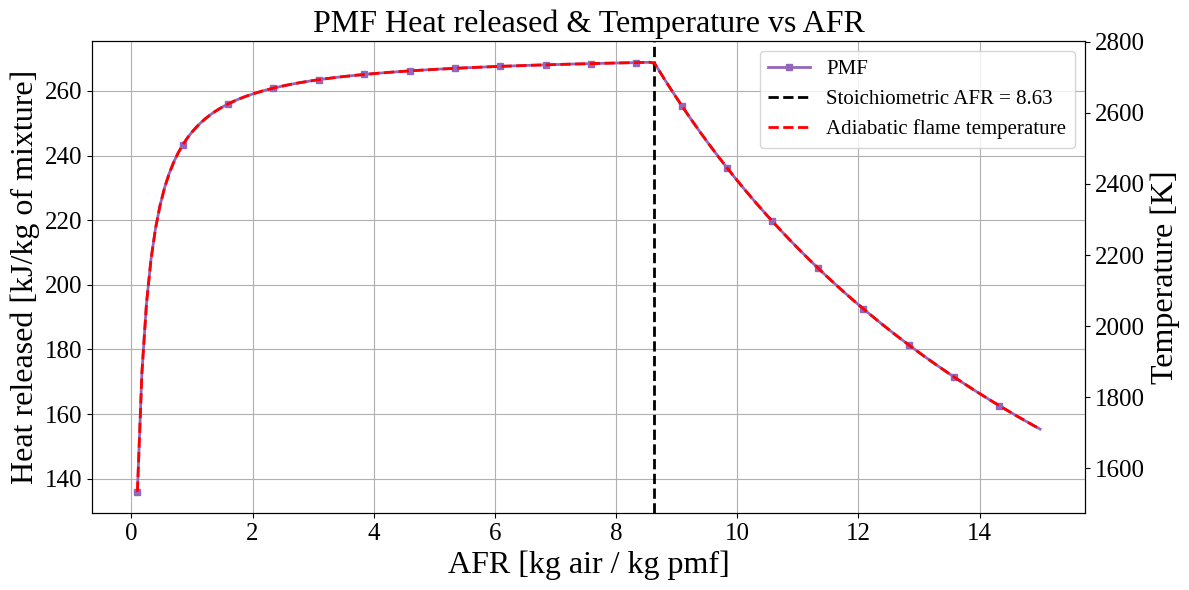
\includegraphics[width=\columnwidth]{FIGURES/respmfafrtimes6.png}
    \caption{Heat released and adiabatic flame temperature per unit mass of mixture as a function of AFR for PMF combustion. The solid curve represents the energy released (kJ/kg of mixture) and temperature (K), while the vertical line marks the stoichiometric AFR, calculated as 8.63~kg~air/kg~PMF for this fuel's composition.}
    \label{fig:PalmisteHeatAFR}
\end{figure}


Figure~\ref{fig:PalmisteHeatAFR} shows how the heat released and temperature per unit mass of fuel-air mixture varies with the AFR for PMF combustion. Maximum heat release occurs at the stoichiometric point, where the oxygen supply exactly matches the demand for complete combustion. Below this value (fuel-rich regime), combustion is incomplete due to oxygen deficiency, limiting energy output. Above the stoichiometric point (air-rich regime), excess air (mainly inert nitrogen) absorbs heat without contributing to the reaction, diluting the thermal energy and reducing specific heat release.\\

Likewise, the adiabatic flame temperature for PMF increases over time, reaching a maximum of approximately 2,700 K. Its temporal behavior follows the heat-release trend, as the temperature rise is directly linked to the energy liberated during combustion.\\

This behavior arises from the interaction between oxygen availability and reaction completeness. When the AFR falls below the stoichiometric value, insufficient oxygen limits the oxidation of carbon and hydrogen, leading to incomplete combustion and lower heat release. Conversely, when AFR exceeds the stoichiometric requirement, the added air—largely inert nitrogen—absorbs part of the generated heat and increases the mixture mass, thereby reducing the specific energy released per unit mass. The sharp decline in heat beyond the stoichiometric point thus reflects a dilution effect rather than a reduction in chemical energy.


\subsubsection{Temporal evolution of chemical species during EFB combustion}\\
\label{sec:EFB_species_evolution}
\begin{figure}[H]
    \centering
    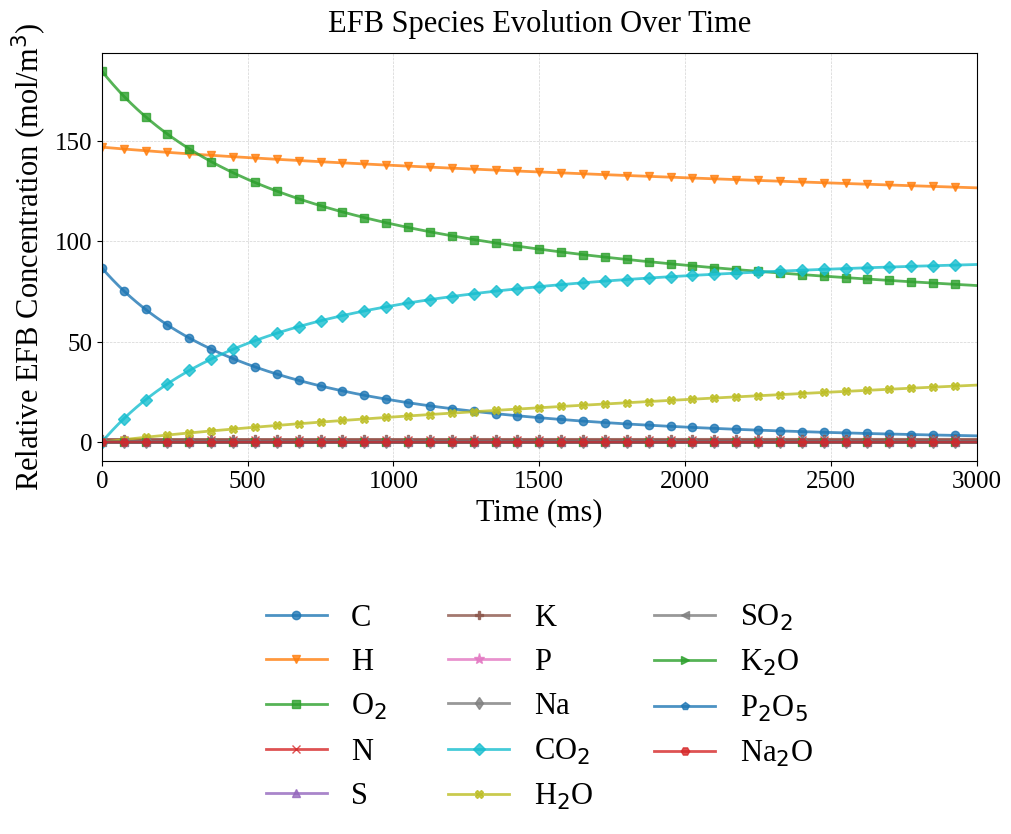
\includegraphics[width=\columnwidth]{FIGURES/resefbcombustion13.png}
    \caption{Species concentration profiles during EFB combustion.}
    \label{fig:EFBConcentracion}
\end{figure}


Figure \ref{fig:EFBConcentracion} shows the relative concentration profiles of chemical species over time throughout the EFB combustion process, capturing the consumption of all reactants and the generation of products. Denoted with line types and colors, three main curves with a decreasing trend present the reduction of reactants that make up almost the 95\% of the mixture (C, H and O$_2$). However, C concentration reduces to zero after 3,000~ms. In the context of the study, the total depletion of C indicates an efficient combustion, as it implies the absence of residual C-based ash at the end of the process. It validates that kinetic reaction constants chosen for EFB combustion are accurate. Similarly, while C, H and O$_2$ diminish, the concentration of combustion compounds CO$_2$ and H$_2$O reach their 80\% concentration formation by millisecond 1500, compensating the initial conditions of the reactants and reflecting the conversion of chemical energy into more stable compounds.\\

In contrast to PMF, EFB contains higher concentrations of alkali elements, specifically K, Na, and P, as reported in Table \ref{tab:composition2_transposed}. During combustion, these elements form inorganic oxides such as K$_2$O, Na$_2$O, and P$_2$O$_5$, which volatilize and are transported as aerosols. Their subsequent deposition on cooler metallic surfaces initiates redox reactions that contribute to alkaline corrosion \cite{BayonaRaquis}. Additionally, the presence of S in the EFB composition facilitates the formation of SO$_2$ and, under condensation conditions, H$_2$SO$_4$, resulting in acidic corrosion \cite{BayonaRaquis}. These mechanisms are consistent with the trends observed in the kinetic evolution curves, where the thermal decomposition of EFB components promotes the release of these corrosive precursors.\\

This behavior aligns with the broader patterns described for biomass-fueled boilers, where corrosion is predominantly driven by the presence of alkali metals and chlorine in the fuel. As detailed by some studies, the volatilized alkali chlorides (such as KCl and NaCl) formed during combustion can react with protective oxide layers (especially chromia (Cr$_2$O$_3$)) on metal surfaces, producing volatile chromates and leading to the loss of protective barriers \cite{BayonaRaquis}. This promotes what is known as “active oxidation,” a mechanism where metal surfaces undergo accelerated degradation through the formation of porous and non-adherent oxide layers. Particularly in super-heater tubes, where gas temperatures and residence times are higher, these interactions can cause significant metal wastage, pitting, and internal oxidation \cite{BayonaRaquis}. Moreover, the synergistic effect of chlorine, alkali metals, and sulfur results in eutectic mixtures with low melting points that exacerbate slag formation and corrosion at localized hotspots. This explains why ferritic steels exposed to high-Cl biomass like EFB may suffer premature failure unless mitigation strategies such as fuel additives or advanced coatings are employed \cite{Mudgal2014}.\\

Although these mechanisms have been documented in the literature, the model developed here provides first-order approximation of the relative formation of corrosive precursors. The simulated temporal profiles of SO$_2$, K$_2$O, Na$_2$O, and P$_2$O$_5$ reveal the general tendency of each biomass to release acid- or alkali-forming species during combustion. These results can serve as reference indicators for future experimental work aimed at quantifying these compounds more precisely and evaluating their implications for material degradation in boiler materials. 

\subsubsection{Energy release and power profile during EFB combustion}
\label{Energy release and power profile during EFB combustion}\\

\begin{figure}[H]
    \centering
    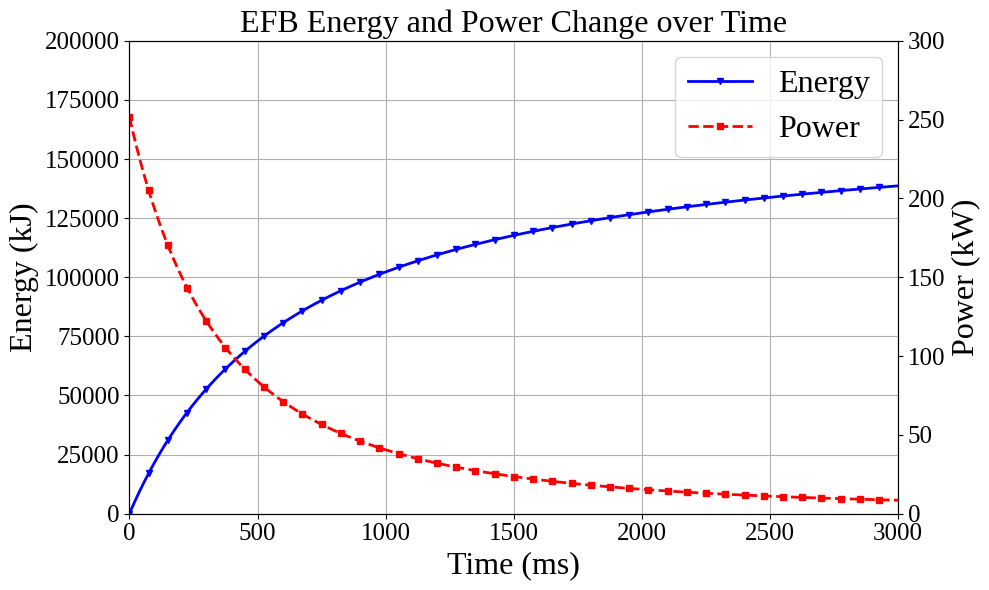
\includegraphics[width=\columnwidth]{FIGURES/resefbenergytimes3.png}
    \caption{Energy and power output during EFB combustion. The solid line denotes the total energy released, while the dashed line illustrates the instantaneous power (rate of energy release).}
    \label{fig:EFBEnergy}
\end{figure}

Figure~\ref{fig:EFBEnergy} presents the combustion energy and corresponding power output for EFB. This energy curve indicates that EFB combustion leads to a total energy release of approximately 140,000~kJ (140~MJ) under the given conditions. A rapid increase occurs during the first 1000~ms, after which the energy gain becomes progressively slower, suggesting a diminishing rate of chemical conversion as volatiles are depleted and fixed carbon combustion completes. This value of released energy is consistent with the result reported by Olisa Y.P. (2014) in \cite{Olisa2014}, where a total of 840 kg of EFB with a similar LHV produced approximately 16,170,000~kJ (16,170~MJ) of energy. The consistency arises from the proportionality of biomass used: the present study employs nearly 1\% of the biomass used in \cite{Olisa2014}, which leads to about 0.8\% of the energy released in Olisa Y.P. study. This proportional match between biomass input and energy output provides an independent validation of the model energy prediction capability. \\

The power profile exhibits a exponential decay, with a peak value close to 250~kW at the onset of combustion. This peak corresponds to the oxidation of volatiles and available surface-bound carbon. As the reaction proceeds, the combustion rate (and therefore power output) drops below 100~kW after 500~ms and continuing to decay to less than 20~kW by the end of the simulated window.\\

This power output can also be compared against the experimental value reported in \cite{Olisa2014}, which indicates a total power release of approximately 1,500~kW from the combustion of 840~kg of EFB. Based on the proportional relationship discussed previously, the present study (using nearly 1\% of the biomass) would be expected to yield a power output in the range of 1\% of the value reported in \cite{Olisa2014}. The peak power value obtained in this simulation corresponds to approximately 16.6\% of the reported value, which remains within a reasonable range considering both studies apply different LHV for EFB and distinct modelling assumptions. This agreement supports the consistency of the power estimation and further validates the energy conversion trends captured by the present model.\\


\subsubsection{Effect of AFR on heat release and adiabatic temperature during EFB combustion}
\label{Heat release variation with AFR during EFB combustion}\\

\begin{figure}[H]
    \centering
    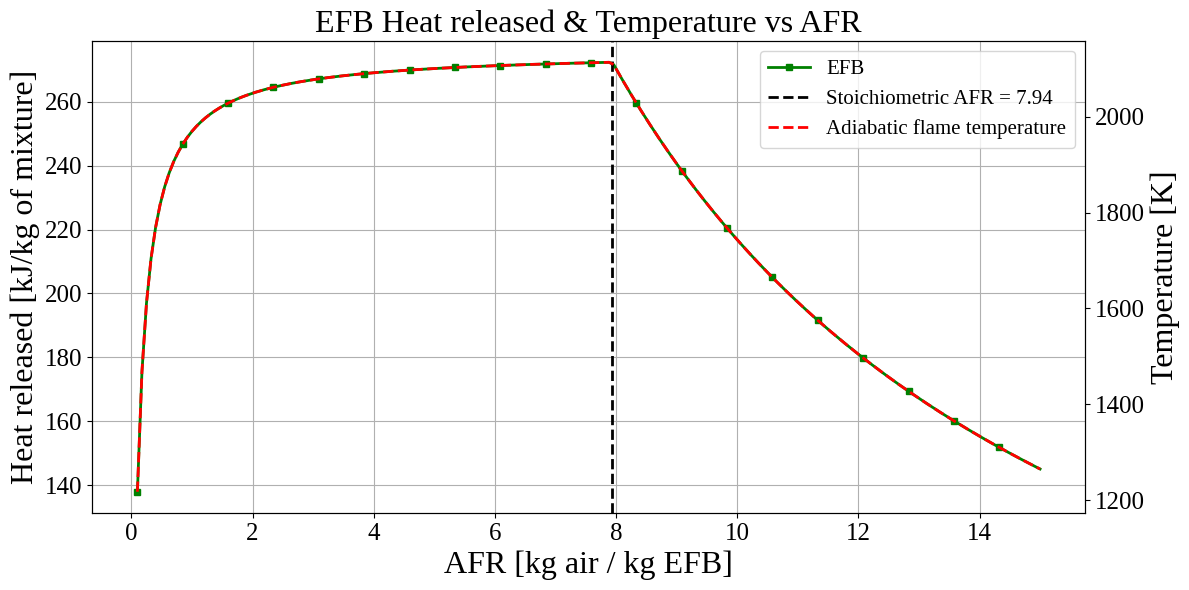
\includegraphics[width=\columnwidth]{FIGURES/resefbafrtimes2.png}
    \caption{Heat released and adiabatic temperature per unit mass of mixture as a function of AFR for EFB combustion. The solid curve represents the total heat released and temperature per kilogram of fuel–air mixture (kJ/kg), while the vertical line indicates the stoichiometric AFR, calculated as 7.94~kg air/kg EFB for this biomass composition.}
    \label{fig:EFBHeatAFR}
\end{figure}


Figure~\ref{fig:EFBHeatAFR} illustrates the relationship between the AFR and the total heat released and temperature per unit mass during the combustion of EFB. The stoichiometric AFR, calculated as 7.94~kg~air/kg~EFB, is marked by a vertical dashed line. The curve exhibits a clear peak at this point, confirming that the stoichiometric ratio ensures the balance between fuel and oxidizer for complete combustion, making it the optimal point.\\

A similar behavior to that observed for PMF in Figure~\ref{fig:PalmisteHeatAFR} is evident in EFB combustion. Sub-stoichiometric conditions limit complete oxidation due to insufficient oxygen, whereas excess-air conditions introduce additional nitrogen and unreacted oxygen that absorb heat and increase the mixture’s mass, thereby reducing specific energy release.\\

With respect to the adiabatic flame temperature, EFB reaches a maximum of approximately 2,500 K at its stoichiometric AFR, while PMF reaches around 2,700 K. This indicates that PMF attains higher adiabatic temperatures under increased air availability, whereas EFB achieves its peak temperature—about 200 K lower—with a reduced air supply.

The temperatures obtained in this analysis exceed typical biomass boiler operating limits. This outcome is expected because they represent adiabatic flame temperatures, which assume idealized conditions with no heat losses. The present model does not account for convective or radiative losses, wall heat transfer, or cooling effects. Although these temperatures do not correspond to real boiler operation, they provide an upper bound on the thermal potential of each fuel under perfectly insulated conditions.

\subsubsection{Effect of Moisture Content on Energy Performance}
\label{Moisture Content}

\textcolor{blue}{Note that this study is conducted on a dry basis, without accounting for the intrinsic moisture content of EFB (48.49\%~\cite{BayonaRaquis}) or PMF (7.8\%~\cite{Pereira2020}). Incorporating moisture introduces an additional endothermic demand associated with heating the water to its boiling point and subsequently vaporizing it, a process that absorbs significant energy and decreases the net heat available for gas heating. By adopting a dry basis, the model isolates the intrinsic chemical energy of the fuel, independent of moisture-induced thermal penalties. \\

To illustrate this effect, two comparative analyses are performed for PMF and EFB by incorporating their respective moisture contents into the total energy balance. The results are shown in Figures~\ref{fig:PMF_moisture} and~\ref{fig:EFB_moisture}. These comparisons are not part of the base simulation model but serve to highlight the energetic relevance of the drying step before combustion.\\


\begin{figure}[H]
    \centering
    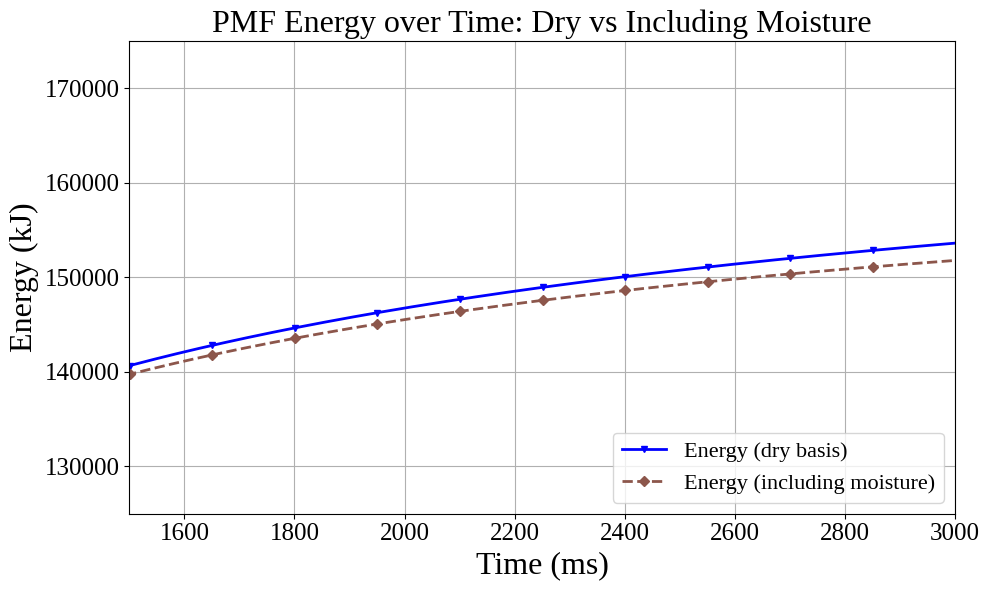
\includegraphics[width=\columnwidth]{FIGURES/respmfmoisture.png}
    \caption{Comparison of energy evolution for PMF under dry basis and when moisture is included in the energy balance.}
    \label{fig:PMF_moisture}
\end{figure}

In Figure~\ref{fig:PMF_moisture}, the energy evolution of PMF is compared under both dry and wet conditions. The curve corresponding to the dry basis reaches 155,000~kJ, as explained in section~\ref{Energy release and instantaneous power output during PMF combustion}, while the curve including moisture follows the same trend up to 1500~ms and then attains 152,000~kJ. The difference between both conditions represents approximately 1.93\% of the total released energy. This reflects the heat consumed by water evaporation instead of contributing to gas-phase heating.\\


\begin{figure}[H]
    \centering
    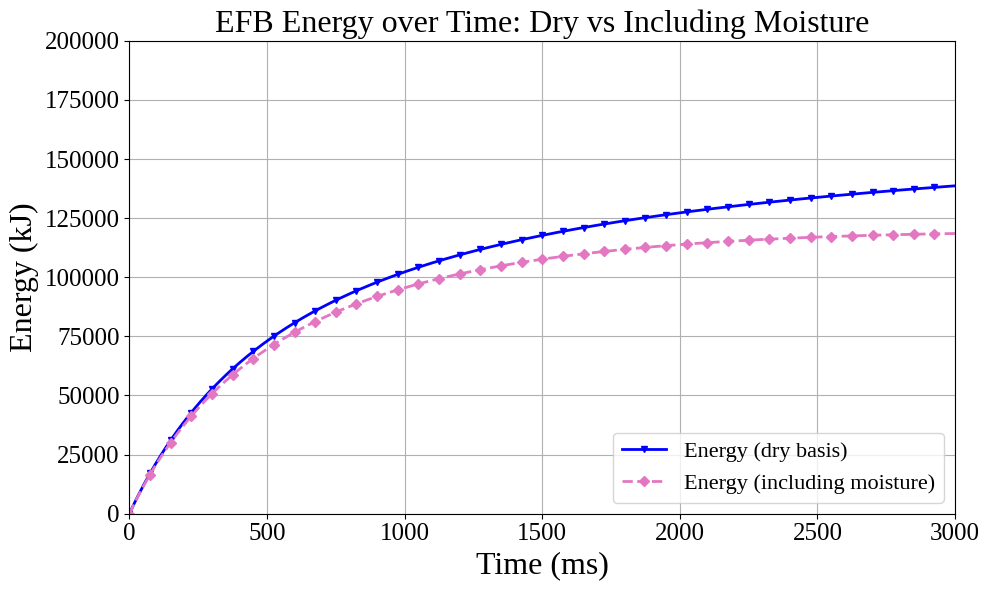
\includegraphics[width=\columnwidth]{FIGURES/resefbmoisture.png}
    \caption{Comparison of energy evolution for EFB under dry basis and when moisture is included in the energy balance.}
    \label{fig:EFB_moisture}
\end{figure}

Figure~\ref{fig:EFB_moisture} presents the corresponding comparison for EFB. Under dry basis, conbustion yields about 140{,}000~kJ, as reported in section~\ref{Energy release and power profile during EFB combustion}, whereas incorporating moisture reduces this value to approximately 120{,}000~kJ. The deviation between both curves corresponds to a reduction of about 15.3\% in the total energy output. The energy loss is about 20~MJ in EFB due to its higher inherent moisture, which increases the proportion of latent heat absorbed during vaporization.\\


From these results, it is observed that the inclusion of moisture content decreases the available energy for both biomasses. This reduction confirms the importance of a drying stage before combustion, ensuring that the system operates near the theoretical conditions assumed in the model.



\subsection{Comparisson between PMF and EFB}
\label{Feasibility comparison between PMF and EFB}

With the model validated and its results established, the next step is to assess the relative feasibility of using each biomass in industrial boiler applications.\\
\begin{figure}[H]
    \centering
    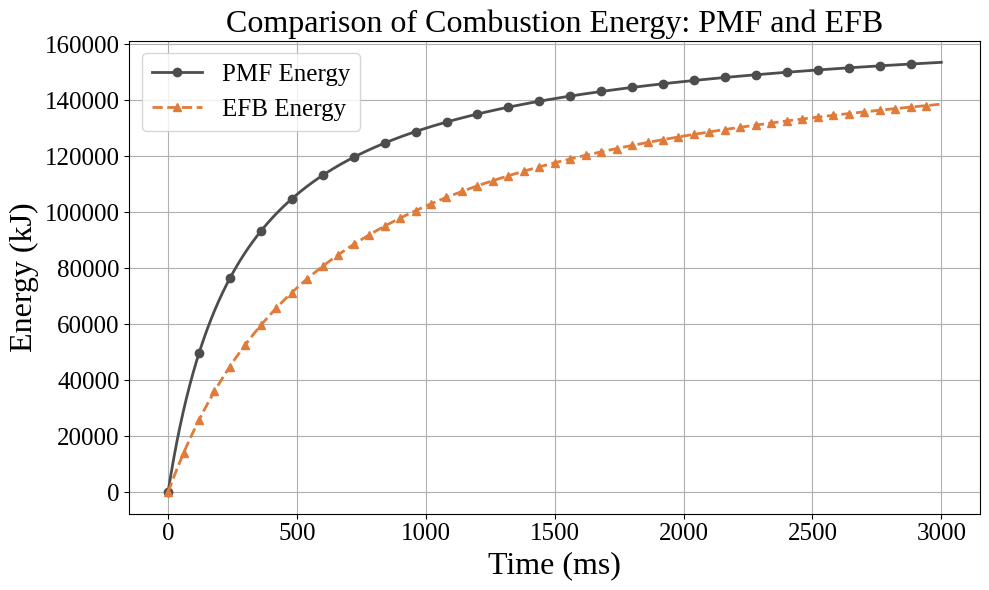
\includegraphics[width=\columnwidth]{FIGURES/resenergycomparison6.png}
    \caption{Energy output comparison between EFB and PMF combustion. The solid line denotes the total energy released by PMF, while the dashed line illustrates the total energy released by EFB.}
    \label{fig:Energycomparison}
\end{figure}


Figure \ref{fig:Energycomparison} offers a comparison of the energy released by both biomass types. Over the same time span, PMF generates approximately 10~MJ more energy than EFB. During the first 500 milliseconds, this energy gap widens steadily, with PMF reaching each energy threshold earlier than EFB, at one point requiring up to 250 milliseconds less. Beyond 500 milliseconds, the time advantage continues to grow: by millisecond 1,000, PMF surpasses 130~MJ, while EFB remains around 100~MJ. The most pronounced time gap is observed at millisecond 1,500, where PMF reaches 140 MJ, whereas EFB requires nearly twice as much time to achieve the same energy output. These results position PMF as the more efficient fuel for energy production, since a difference amount of energy released per unit of biomass results in usable power and may reduce the amount of fuel required to meet a given energy demand. However, this advantage is directly linked to the quantity of residue generated from the oil palm industry.\\

Compared to PMF, the total energy output of EFB reaches approximately 140~MJ, while PMF reaches 150~MJ under the same combustion conditions. This difference aligns with the values reported in section \ref{energy_section}, where EFB shows a LHV of 17.66~MJ/kg, compared to 19~MJ/kg for PMF; however, other sources indicate overlapping ranges, suggesting that both materials can exhibit comparable energy content depending on moisture and ash content. Regarding the power profiles, the peak power of EFB is approximately 250~kW, whereas PMF reaches 600~kW. After the initial 500~ms, EFB power output decreases below 100~kW and drops under 20~kW by the end of the process, while PMF maintains values above 25 kW for the 3,000~ms.\\

\begin{figure}[H]
    \centering
    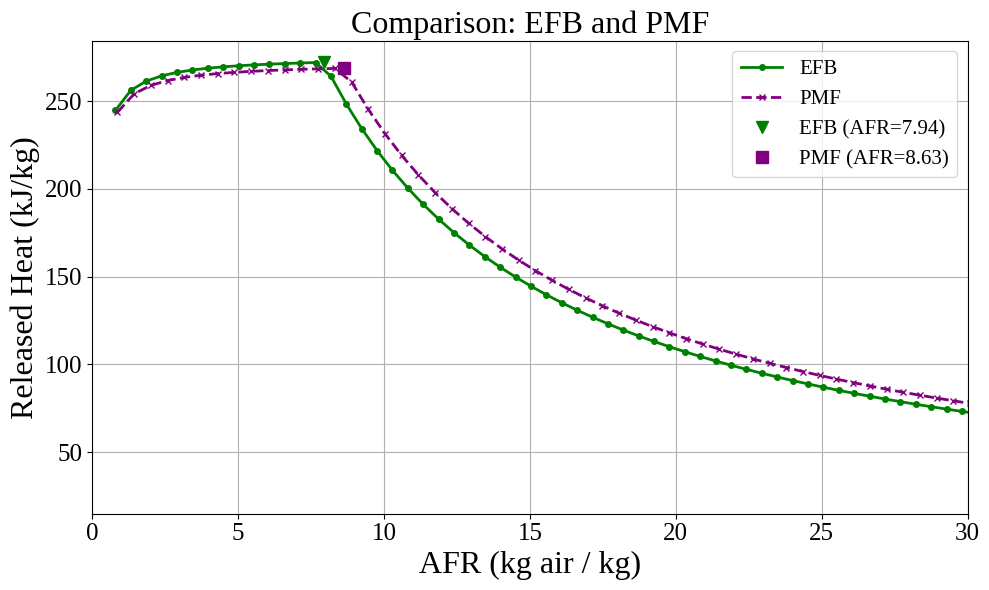
\includegraphics[width=\columnwidth]{FIGURES/rescomparisontimes.png}
    \caption{Comparison of heat released as a function of AFR for EFB and PMF combustion. The curves represent the heat released for EFB and PMF, respectively. The plot highlights the shift in optimal AFR and the different sensitivity to excess air conditions between the two biomasses.}
    \label{fig:compAFR}
\end{figure}

Figure~\ref{fig:compAFR} shows the comparison of heat release as a function of AFR for EFB and PMF. EFB reaches its maximum heat release at an AFR of 7.94~kg~air/kg~fuel, while PMF reaches its peak at 8.63~kg~air/kg~fuel. This difference is consistent with the distinct elemental compositions of both fuels, as discussed in previous sections. Under stoichiometric conditions, both biomasses release comparable amounts of energy: 275~kJ/kg for EFB and 265~kJ/kg for PMF. Beyond the optimal AFR, the heat output of EFB decreases more sharply, reaching 75~kJ/kg at 30~kg~air/kg~fuel, whereas PMF maintains 80 kJ/kg under the same conditions. In contrast, under sub-stoichiometric conditions, EFB achieves 90\% of its peak heat release at an AFR of 4~kg~air/kg~fuel, while PMF requires 7~kg~air/kg~fuel to reach the same proportion.  These results indicate that EFB delivers a higher fraction of its energy at lower AFR, but loses heat release capacity faster under excess-air conditions compared to PMF.\\

Both fuels exhibit the same general trend: heat release decreases under oxygen-deficient conditions due to incomplete combustion and under excess-air conditions due to thermal dilution.\\

The AFR behavior of EFB may be advantageous in combustion systems where airflow is constrained or where minimizing excess air is a priority. \\




%Last, as noted in the introduction, EFB and PMF account for approximately 20\% and 13\% \cite{BayonaRaquis} of the total residues produced by the Colombian palm oil sector, respectively. According to Fedepalma, Colombia generates more than 1.5 million tons of EFB per year \cite{Fedepalma2023}. Based on the aforementioned percentages, the estimated annual production of PMF is around 0.975 million tons; consequently, the difference in the generated residues of EFB and PMF is over 0.525 million tons. When this difference in availability is considered alongside the comparable energy output observed in combustion tests and the better performance of EFB under lower AFR conditions, the total recoverable energy from EFB becomes significantly greater in large-scale applications.\\

%Given the relatively similar total energy output of both biomasses, the greater availability of EFB, and its superior performance under optimal AFR conditions, it is recommended to prioritize EFB for biomass boiler applications. Meanwhile, PMF may be better allocated to other profitable uses.\\

%%%%%%%%%%%%%%%%%%%%%%%%%%%%%%%%%%%%%%%%%%%%%%%%%%%%%%

\section{Conclusions}\label{conclusions}

This study presents a combustion model as dynamic chemical species transformations of EFB and PMF in time. The structure, defined by a system of ODE, provides a consistent and adaptable framework for simulating the evolution of reactants and products under controlled air-fuel conditions. Its structure supports real-time adjustment of parameters such as biomass composition, AFR, and reaction kinetics. The model also provides combustion time-predictions and includes calibrated kinetic constants for EFB and PMF, facilitating fast scenario analysis and practical integration into biomass energy applications. \\

Model validation is achieved by comparing the simulated energy outputs against theoretical values derived from the LHV of each biomass. For PMF, the model yielded 150~MJ compared to 158.27~MJ theoretical, resulting in a relative error of 5.51\%, while for EFB the simulation reported 140~MJ against 147.11~MJ, with a 5.07\% error (as detailed in section~\ref{Validation of the model}).\\

Regarding biomass performance, EFB achieved its maximum heat release at a lower AFR than PMF and delivered more energy per unit of air at that point (as reported in section~\ref{Feasibility comparison between PMF and EFB}). The combination of better stoichiometric performance and greater annual availability makes dry EFB a strong candidate for substitution in biomass boilers operating with PMF.\\

%Beyond combustion modeling, the results obtained have direct implications for biomass boiler design and operation. By incorporating EFB as a primary fuel and reallocating PMF to applications better suited to its physical characteristics, total energy generation in biomass boilers can increase by up to 30\%. This improvement stems not from higher energy content per unit of fuel, but from a more efficient use of available residues within the palm oil sector. The favorable AFR performance of EFB further supports its integration into boiler systems without requiring additional mass flow or excessive air injection, paving the way for more compact combustion chambers and better control over heat transfer dynamics.\\

%The feasibility of using EFB as biofuel in boilers also entails specific technical considerations. Its combustion produces compounds such as SO$_2$ and the formation of H$_2$SO$_4$, which can lead to acid corrosion, as well as alkali oxides (K$_2$O, Na$_2$O, P$_2$O$_5$) responsible for alkaline corrosion of metal surfaces. To prevent these compounds from reaching heat exchangers and other thermal components, it is necessary to ensure their condensation and solidification inside the combustion chamber, where they can be retained in ash form at the grate level. This may be achieved by managing air injection temperatures and flow distribution, so that corrosive vapors cool and settle before being entrained by the exhaust flow. Future studies could evaluate optimized multi-zone configurations to enhance this retention mechanism and minimize corrosion risks throughout the system.\\

The implications identified in this work are consistent with recommendations from the oil palm context, where the need for multi-zone combustion, staggered air injection, and thermal control has been highlighted to reduce corrosion and improve EFB utilization in industrial boilers~\cite{BayonaRaquis}. The proposed model provides a flexible computational framework to quantify compounds such as SO$_2$ and the formation of H$_2$SO$_4$, which can lead to acid corrosion, as well as alkali oxides (K$_2$O, Na$_2$O, P$_2$O$_5$) responsible for alkaline corrosion of metal surfaces.\\

The proposed model can be generalizable to other biomasses, provided that their elemental composition and LHV are known. Its formulation allows seamless integration into CFD frameworks to simulate species transport and combustion dynamics, which is essential for spatially resolving thermal behavior, emissions, and reaction zones inside industrial biomass systems.\\


When incorporated into a CFD environment capable of solving the Navier–Stokes equations, turbulence, and energy transport, the proposed kinetic model can supply a consistent description of EFB combustion within boiler-scale domains. Such coupling would enable the prediction of temperature fields, gas velocities, and reactive species distribution, supporting the optimization of air-injection strategies and thermal-management schemes in industrial biomass systems.\\

Note that, as discussed earlier in the manuscript, the present model could not be fully calibrated due to the absence of TGA or DTG or published kinetic constants for EFB. Without experimental reaction times or heat-release curves, the analysis of kinetic-parameter sensitivity and the minimization of LHV error cannot yet be performed. For this reason, the current model offers a physically coherent first approximation rather than a fully validated kinetic mechanism.\\

Looking forward, experimental combustion measurements will make it possible to identify realistic kinetic constants and conduct rigorous uncertainty and sensitivity analyses. With those datasets, the present kinetic model could be transformed into a high-fidelity kinetic module suitable for direct integration into CFD tools, ultimately enabling more accurate predictive simulations and supporting future design and optimization of biomass boilers operating with EFB.\\
%%%%%%%%%%%%%%%%%%%%%%%%%%%%%%%%%%%%%%%%%%%%%%%%%%%%%%%
\section{Declarations}

\subsection{Declaration of competing interest}
The authors declare that they have no known competing financial interests or personal relationships that could have appeared to influence the work reported in this paper.

\subsection{Funding}
This research did not receive any specific grant from funding agencies in the public, commercial, or not-for-profit sectors.

\subsection{Author Contributions}

\textbf{Arias-Guerrero, D.A.}: Data curation, Formal analysis, Investigation, Methodology, Resources, Software, Supervision, Validation, Writing – original draft. \textbf{Castillo-Hernández, M.A.}: Data curation, Investigation, Resources, Visualization, Writing – original draft. \textbf{Mayorga-Guzmán, J.D.}: Data curation, Formal analysis, Investigation, Resources, Visualization, Writing – original draft. \textbf{Bayona Roa, C.A.}: Conceptualization, Data curation, Methodology, Project administration, Resources, Supervision, Writing – review and editing. 




%%%%%%%%%%%%%%%%%%%%%%%%%%%%%%%%%%%%%%%%%%%%%%%%%%%%%%%

%% For citations use: 
%%       \cite{<label>} ==> [1]

%%
%Example citation, See \cite{lamport94}.

%% If you have bib database file and want bibtex to generate the
%% bibitems, please use
%%
%%  \bibliographystyle{elsarticle-num} 
%%  \bibliography{<your bibdatabase>}

%% else use the following coding to input the bibitems directly in the
%% TeX file.

%% Refer following link for more details about bibliography and citations.
%% https://en.wikibooks.org/wiki/LaTeX/Bibliography_Management
\bibliographystyle{elsarticle-num}
\begin{thebibliography}{00}

%% For numbered reference style
%% \bibitem{label}
%% Text of bibliographic item

\bibitem{FAOSTAT2024}
Food and Agriculture Organization of the United Nations.
\textit{World Food and Agriculture – Statistical Yearbook 2023}.
FAO, Rome, 2023.
DOI: \href{https://doi.org/10.4060/cc8166en}{https://doi.org/10.4060/cc8166en}.
(Accessed 1 Aug 2025).

\bibitem{USDA2024}
United States Department of Agriculture, Foreign Agricultural Service.
\textit{Oilseeds: World Markets and Trade – January 2024}.
USDA FAS, January 2024.
Available at
\href{https://apps.fas.usda.gov/PSDOnline/}{https://apps.fas.usda.gov/PSDOnline/}.
(Accessed 1 Aug 2025).


%\bibitem{Agronet} Fedepalma, La palma de aceite colombiana en cifras, balance 2022 y retos 2023 (Feb. 2023). \url{https://www.agronet.gov.co/Noticias/Paginas/La-palma-de-aceite-colombiana-en-cifras%2C-balance-2022-y-retos-2023.aspx} (accessed April 9, 2025).

\bibitem{BayonaRaquis} C. Bayona-Roa, J.G. García-Navarro, J. Gacha, H. Ricaurte, Hacia el aprovechamiento energético de los raquis de palma en calderas de biomasa, Rev. Palmas. 44(1) (2023) 51--64. \href{https://doi.org/10.56866/01212923.13806}{https://doi.org/10.56866/01212923.13806}.




\bibitem{Fedepalma2023}
Fedepalma, Informe de gestión 2023 (2023)
\href{https://publicaciones.fedepalma.org/index.php/labfedepalma/article/view/14221/14100}
{https://publicaciones.fedepalma.org/index.php/labfedepalma/article/\\view/14221/14100}
(accessed March 2025).

%%%%%%%%%%%%%%%%%%%%%%%%%%%%%%%%%%%%%%%%%%%%

\bibitem{NacionesUnidasMetano} Programa de las Naciones Unidas para el Medio Ambiente, Datos sobre el metano (n.d.). \href{https://www.unep.org/es/explore-topics/energy/datos-sobre-el-metano}{https://www.unep.org/es/explore-topics/energy/datos-sobre-el-metano} (accessed June 24, 2025).

\bibitem{WanRosli2011} W.R. Wan Daud, K.N. Law, Oil palm fibers as papermaking material: Potentials and challenges, BioResources. 6(1) (2011) 901--917. \href{https://doi.org/10.15376/biores.6.1.901-917}{https://doi.org/10.15376/biores.6.1.901-917}.

\bibitem{Angarita2009} J.D. Angarita Martínez, D.I. Díaz Durán, L.A. Lozano Urbina, Fibra de palma africana (Elaeis guineensis) para mejorar las propiedades mecánicas del cartón reciclado, Rev. ION. 22(1) (2009) 63--71.


\bibitem{Khan2023} T.A. Khan, Y. Yang, R. Kumar, Z. Yu, Kinetics of combustion of lignocellulosic biomass: Recent research, Fuel. 346 (2023) 128423. \href{https://doi.org/10.1016/j.fuel.2023.128310}{https://doi.org/10.1016/j.fuel.2023.128310}.



\bibitem{Ninduangdee2015} P. Ninduangdee, V.I. Kuprianov, E.Y. Cha, R. Kaewrath, P. Youngyuen, W. Atthawethworawuth, Thermogravimetric studies of oil palm empty fruit bunch and palm kernel shell: TG/DTG analysis and modeling, Energy Procedia. 79 (2015) 453--458. \href{https://doi.org/10.1016/j.egypro.2015.11.518}{https://doi.org/10.1016/j.egypro.2015.11.518}.


\bibitem{Jia2021} G. Jia, Combustion characteristics and kinetic analysis of biomass pellet fuel using thermogravimetric analysis, Processes. 9(5) (2021) 868. \href{https://doi.org/10.3390/pr9050868}{https://doi.org/10.3390/pr9050868}.



\bibitem{GarciaNunez2006} J.A. García-Núñez, M. García-Pérez, K.C. Das, Determination of kinetic parameters of thermal degradation of palm oil mill by-products using thermogravimetric analysis and differential scanning calorimetry, in: ASABE Annual International Meeting, Portland, Oregon, July 9–12, 2006. \href{https://doi.org/10.13031/2013.21519}{https://doi.org/10.13031/2013.21519}.



\bibitem{Dhahak2021} A. Dhahak, R. Bounaceur, C. Le Dreff-Lorimier, G. Schmidt, G. Trouvé, F. Battin-Leclerc, Development of a detailed kinetic model for the combustion of biomass, Fuel. 306 (2021) 121668. 



\bibitem{Ranzi2013} E. Ranzi, M. Corbetta, F. Manenti, S. Pierucci, Kinetic modeling of the thermal degradation and combustion of biomass, Chem. Eng. Sci. 110 (2013) 2–12. \href{https://doi.org/10.1016/j.ces.2013.08.014}{https://doi.org/10.1016/j.ces.2013.08.014}.



\bibitem{Luo2019} H. Luo, Modelling of biomass combustion and gasification: From particle-scale to reactor-scale, Ph.D. Thesis, Technical University of Denmark, 2019.




\bibitem{Frank2014} A. Frank, M.J. Castaldi, CFD analysis of municipal solid waste combustion using detailed chemical kinetic modelling, Waste Manag. Res. 32(8) (2014) 745–754. \href{https://doi.org/10.1177/0734242X14538305}{https://doi.org/10.1177/0734242X14538305}.


\bibitem{Silva2023} J. Silva, S. Teixeira, J. Teixeira, A review of biomass thermal analysis, kinetics and product distribution for combustion modeling: From the micro to macro perspective, Energies. 16(18) (2023) 1--39. \href{https://doi.org/10.3390/en16186705}{https://doi.org/10.3390/en16186705}.


\bibitem{Navarrete2017} G. Navarrete, P. Curto-Risso, W.A. Bizzo, Simplified model and simulation of biomass particle suspension combustion in one-dimensional flow applied to bagasse boilers, Biomass Bioenergy. 99 (2017) 38--48. \href{https://doi.org/10.1016/j.biombioe.2017.01.030}{https://doi.org/10.1016/j.biombioe.2017.01.030}.

\bibitem{Varhegyi2020} G. Várhegyi, L. Wang, Ø. Skreiberg, Empirical kinetic models for the combustion of charcoals and biomasses in the kinetic regime, Energy Fuels. 34(10) (2020) 12327--12345. \href{https://doi.org/10.1021/acs.energyfuels.0c03248}{https://doi.org/10.1021/acs.energyfuels.0c03248}.




\bibitem{OilPalmRachisGasification} J.C. Solarte Toro, Oil palm rachis gasification for synthesis gas production, Undergraduate Thesis, Universidad Nacional de Colombia, Sede Manizales, Facultad de Ingeniería y Arquitectura, Departamento de Ingeniería Química, 2017.





\bibitem{Ramos2017} D. Flórez Ramos, Obtención de gas de síntesis a partir de la gasificación de cuesco de palma de aceite peletizado, Undergraduate Thesis, Universidad Nacional de Colombia, Sede Bogotá, Facultad de Ingeniería, Departamento de Ingeniería Química y Ambiental, 2017. \href{https://repositorio.unal.edu.co/handle/unal/60817}{https://repositorio.unal.edu.co/handle/unal/60817}.



%%%%%%%%%%%%articulos de modelos cineticos%%%%%%
\bibitem{Dhaundiyal2019} 
R. Dhaundiyal, A. Singh, R. Tewari, Thermo-kinetics of forest waste using model-free methods, 
Ingeniería y Competitividad 21(1) (2019) 1--12. 
\href{http://www.scielo.org.co/scielo.php?script=sci_arttext&pid=S0122-74832019000100001}{http://www.scielo.org.co/scielo.php?script=sci_arttext&pid=S0122-74832019000100001}.

\bibitem{DiCelso2014} 
F. di Celso, N. De Blasio, G. Ruoppolo, A. Cavaliere, R. Ragucci, 
Kinetics of pyrolysis and combustion of spherical wood, 
Energy 74 (2014) 104--118. 
\href{https://doi.org/10.1016/j.energy.2014.02.047}{https://doi.org/10.1016/j.energy.2014.02.047}.

%%%%%%%%%%%%%%%%%%%%%%%%%%%%%%%%%%%%%%%%%%%%%%%%

\bibitem{Idris2012} S.S. Idris, N.A. Rahman, K. Ismail, Combustion characteristics of Malaysian oil palm biomass, sub-bituminous coal and their respective blends via thermogravimetric analysis (TGA), Bioresour. Technol. 123 (2012) 581--591. \href{https://doi.org/10.1016/j.biortech.2012.07.065}{https://doi.org/10.1016/j.biortech.2012.07.065}.

\bibitem{Olisa2014} Y.P. Olisa, K.W. Kotingo, Utilization of palm empty fruit bunch (PEFB) as solid fuel for steam boiler, Eur. J. Eng. Technol. 2(2) (2014).



\bibitem{Madhiyanon2012} T. Madhiyanon, P. Sathitruangsak, S. Sungworagarn, S. Pipatmanomai, S. Tia, A pilot-scale investigation of ash and deposition formation during oil-palm empty-fruit-bunch (EFB) combustion, Fuel Process. Technol. 96 (2012) 250--264. \href{https://doi.org/10.1016/j.fuproc.2011.12.020}{https://doi.org/10.1016/j.fuproc.2011.12.020}.



\bibitem{Ramirez2011} C. Ramírez, E. Nidia, E.M. Garzón, R. Silva, S. Ángela, A. Yáñez, E. Edgar, Caracterización y manejo de subproductos del beneficio del fruto de palma de aceite, 2011.




\bibitem{Kaniapan2021} S. Kaniapan, S. Hassan, H. Ya, K. Patma Nesan, M. Azeem, The utilization of palm oil and oil palm residues and the related challenges as a sustainable alternative in biofuel, bioenergy, and transportation sector: A review, Sustainability. 13(6) (2021) 3110. \href{https://doi.org/10.3390/su13063110}{https://doi.org/10.3390/su13063110}.



\bibitem{NISTkinetics} National Institute of Standards and Technology, NIST Chemical Kinetics Database, U.S. Department of Commerce, 2025 \href{https://kinetics.nist.gov/kinetics/}{https://kinetics.nist.gov/kinetics/} (accessed July 15, 2025).


\bibitem{AtkinsPChem} P. Atkins, J. de Paula, Atkins' Physical Chemistry, 8th ed., Oxford University Press, Oxford, 2006.

\bibitem{HindmarshODEPACK}
Hindmarsh, A. C. \textit{ODEPACK, A Systematized Collection of ODE Solvers}. Report UCRL-ID-113855, Lawrence Livermore National Laboratory, 1983. 

\bibitem{Mudgal2014} D. Mudgal, S. Singh, S. Prakash, Corrosion problems in incinerators and biomass-fuel-fired boilers, Int. J. Corros. 2014 (2014) Article ID 505306, 14 pages. \href{https://doi.org/10.1155/2014/505306}{https://doi.org/10.1155/2014/505306}.


\bibitem{Pereira2020} P.H.F. Pereira, N.F. Souza, H.L. Ornaghi, M.R. de Freitas, Comparative analysis of different chlorine-free extraction on oil palm mesocarp fiber, Ind. Crops Prod. 150 (2020) 112305. \href{https://doi.org/10.1016/j.indcrop.2020.112305}{https://doi.org/10.1016/j.indcrop.2020.112305}.


\end{thebibliography}

\end{document}

\endinput
%%
%% End of file `elsarticle-template-num.tex'.



\section{Response to reviewers}

This statement concerns the revised version of the manuscript \PaperTitle{\textit{"Computational Modeling of the Combustion Reaction Kinetics of the Oil Palm's Empty Fruit Bunch and Mesocarp Fiber"}} submitted under reference 259208490, prepared in response to the reviewers’ comments.\\

The comments provided by the reviewers have been very useful. Following their suggestions, the manuscript was improved and clarified in several sections. In addition, each comment is addressed individually in the responses below. All modifications are highlighted in \textcolor{blue}{blue color} in the revised manuscript, and each response specifies the section where the corresponding change was introduced.


\subsection{Reviewer 1}

1. The manuscript claims novelty in developing a dynamic kinetic model resolving time-dependent combustion species for EFB and PMF. While the approach is sound, the novelty should be more clearly emphasized by comparing this method against previous semi-empirical and detailed kinetic models in terms of accuracy and computational efficiency. \\

\textcolor{blue}{To clarify the novelty of the approach, the end of the Introduction was revised to explicitly position the proposed model in relation to existing kinetic methods. The updated text now includes a brief comparison with semi-empirical, TGA-based models (which do not resolve species evolution in time) and with detailed kinetic mechanisms that require substantially higher computational cost. This addition highlights that the formulation provides an intermediate alternative by resolving the temporal behavior of multiple reactants and products for EFB and PMF while maintaining computational efficiency. These clarifications strengthen the presentation of the model’s methodological contribution. The new paragraphs have been incorporated in Section~\ref{intro}.}\\



2. The validation is primarily based on energy output comparisons (LHV). Additional discussion on model sensitivity to kinetic parameters and error propagation would enhance scientific robustness. \\

\sloppy
\textcolor{blue}{In response, we have added a dedicated explanation in the revised manuscript clarifying the limitations associated with the kinetic constants and the constraints of the current validation strategy Section~\ref{efbmodelval}. Specifically, we now explain that no calorimetric experiments or published kinetic parameters exist for EFB combustion, which prevents a rigorous sensitivity or error-propagation analysis at this stage. The model is therefore validated using the theoretical LHV as the sole experimental benchmark, ensuring mass and energy consistency but not allowing parameter calibration against time-resolved combustion data.}\\


\textcolor{blue}{The revised text also outlines a future research pathway in which bomb calorimeter measurements and controlled combustion experiments would enable the determination of accurate reaction times, heat-release profiles, and species-conversion rates. With such experimental data, the model can be refined to identify optimal kinetic constants and to perform the full sensitivity and uncertainty analysis suggested by the reviewer. This clarification has been incorporated into the manuscript to explicitly acknowledge the limitation and to strengthen the scientific positioning of the proposed model.\\}
\fussy

3. Authors should discuss possible limitations due to the assumption of constant reaction rate coefficients (temperature-independent) and its implications on generalizability. \\

\textcolor{blue}{Assuming constant reaction rate coefficients constitutes a limitation in terms of accuracy for real combustion processes, as temperature-dependent kinetics would influence the gradients of species molar fractions at specific stages of the reaction. This consideration has now been explicitly discussed in Section~\ref{Kinetic Modelling of Comustion}. At present, no validated temperature-dependent kinetic parameters are available in the literature for EFB or PMF, which restricts the formulation to a simplified representation. For this reason, the model is presented as an initial framework that captures the overall species evolution, while acknowledging that future work should incorporate temperature-dependent rate coefficients. This need for experimentally validated temperature-dependent parameters is also highlighted in the Conclusions as a key direction for further development of the model.\\}

4. The derivation and calibration of kinetic constants from the NIST database are briefly mentioned. More detail is required on how these constants were adjusted for biomass-specific reactions. \\

\textcolor{blue}{Additional detail has been included in Section~\ref{energy_section} to clarify how the kinetic constants derived from the NIST database are adapted for the combustion of EFB and PMF. The revised text explains that the calibration relied on an iterative procedure in which increasing or decreasing the constants accelerated or delayed the consumption of the species, respectively. After each adjustment, the released energy is compared with the theoretical value in order to guide the calibration. The revision also specifies that, throughout this process, the relative order of magnitude among the constants is preserved so that the expected reactivity of each species remained physically coherent (e.g., carbon oxidizing more slowly than hydrogen). This ensured that the calibrated constants maintained realistic reaction behavior while allowing the global heat release to converge toward the theoretical value.}\\


5. It would be beneficial to include a table comparing literature kinetic constants with those used in this study.\\

\textcolor{blue}{After a thorough review, we found that no kinetic constants for the combustion of EFB have been reported in the literature thus far. As a result, it is not currently possible to provide such a comparison.\\}



6. The study assumes dry biomass conditions. While justified, a brief quantitative estimation of how real moisture content could influence combustion efficiency and energy output should be added to strengthen practical relevance. \\

\textcolor{blue}{The observation regarding the assumption of dry biomass conditions was addressed by performing a quantitative estimation of the influence of moisture content on combustion efficiency. According to the proximate analyses of both biomasses, the EFB shows an average moisture content of 48.49 \%, while the PMF presents 7.8\%. Based on these values and using the specific heat and enthalpy of vaporization of water, the amount of heat required to evaporate the inherent moisture was calculated and then subtracted from the total energy released during combustion. The resulting difference represents the net useful energy of the process after accounting for the latent heat of vaporization.}\\

\textcolor{blue}{This estimation provides a quantitative reference for understanding how the initial moisture reduces the effective energy output of the fuel. The main kinetic model, however, was formulated under dry-biomass conditions, consistent with industrial practice where pre-drying processes (such as hot-air drying or natural conditioning) are typically applied prior to combustion. The discussion of this aspect has been incorporated into a new Section~\ref{Moisture Content}.}\\



7. Figures (particularly Figs. 2-9) are informative but require improved labeling (axes units, legends, and clearer distinction between EFB and PMF results). \\

\textcolor{blue}{The graphics have been corrected. Thank you in advance.}\\

8. Consider adding a schematic of the model workflow or computational setup for reader clarity. \\

\textcolor{blue}{Schematic of the model workflow is now added in section 2. Methodology. Thank you for the advice.\\}


9. The section on alkali and sulfur corrosion (page 20-22) is well written but reads like an extended literature review. It could be condensed and directly linked to the model's predictive capability (e.g., can the model estimate the relative concentration of corrosive species?). \\

\textcolor{blue}{In the revised manuscript, the section has been shortened and a paragraph has been added to explicitly link the discussion of alkali and sulfur corrosion to the predictive capability of the model. The text now clarifies that, although the model provides a simplified kinetic representation, it does estimate the relative temporal formation of species such as SO$_2$, K$_2$O, Na$_2$O and P$_2$O$_5$. This information offers an initial indication of the tendency of each biomass to release acid- or alkali-forming compounds, which can serve as a reference for future work aimed at more precise quantification and material-level assessment. This addition strengthens the connection between the simulated species evolution and corrosion precursors, addressing the reviewer’s suggestion. The new text has been added in Section~\ref{sec:EFB_species_evolution}.}\\


10. The conclusion mentions that the model can support boiler design and CFD integration. It would be valuable to provide a short paragraph outlining how this model could be integrated into real industrial systems or used to guide material selection. \\

\textcolor{blue}{A new paragraph outlining how this model could be integrated into real industrial systems or used as a guide material selection has been included in section 4. Conclusions.\\}

11. Some typographical and grammatical errors are present (e.g., "ued" → "used"; "combustion gases composition can be obtaine" → "obtained"). A careful proofreading is recommended. \\

\textcolor{blue}{Typographical and grammatical have been errors corrected. We thanks for highlighting these faults.\\}

12. References should be formatted consistently (some use DOI hyperlinks, others not). \\

\textcolor{blue}{All links now use hyperlinks. Thank you.\\}

13. Please define all abbreviations at first mention (e.g., AFR, LHV). \\

\textcolor{blue}{All abbreviations are now defined at first mention.\\}

14. The abstract could briefly mention the computational method (Python-LSODA solver) earlier to highlight reproducibility. \\

\textcolor{blue}{To address this point, the abstract was revised so that the computational method is mentioned earlier in the first technical sentence. The updated version now specifies that the model was implemented in Python and solved using the LSODA algorithm, which more clearly highlights the reproducibility of the approach. The revised wording has been incorporated into the abstract.}\\

15. Include units wherever necessary (e.g., Table 3 and 4 concentrations, rate constants).\\

\textcolor{blue}{Units have been included in the Tables.}

\subsection{Reviewer 2}

Q1. Only elemental compositions of fuel are input data, while its proximate properties, especially moisture, are also impacted on characteristics of the combustion process. Authors should explain why exclude those properties.\\

\textcolor{blue}{The exclusion of proximate properties, particularly moisture, was based on the modeling assumption of dry biomass, which reflects standard industrial operation where pre-drying of EFB and PMF is performed before combustion. Nevertheless, an additional estimation has been incorporated to quantify the thermal effect of the actual moisture content reported for each biomass (48.49 \% for EFB and approximately 7.8 \% for PMF). Using the specific heat and vaporization enthalpy of water, the heat required for moisture evaporation is calculated and subtracted from the total combustion energy to obtain the net effective energy. This clarification is now included into a new Section~\ref{Moisture Content} to highlight how moisture content affects the overall efficiency without altering the structure of the kinetic model.}\\

Q2. Page 11, Section 2.1.3 “atmospheric air consists of approximately 21\% O2 and 78\% N2”. It would be 79\% N2 to correspond a molar ratio of 1:3.76 for O2 to N2.\\

\textcolor{blue}{The text has been corrected to state that atmospheric air is assumed to contain 21\% O$_2$ and 79\% N$_2$, which is consistent with the commonly used molar ratio of 1:3.76 for O$_2$ to N$_2$ in combustion calculations. The corresponding sentence is now included in Section~\ref{Calculus of the required Oxygen for combustion}.
}\\

Q3. The criteria the authors used to judge convergence are unclear. It appears the reaction process is incomplete at 3000 ms. Can the model's time period be extended to 5000 ms?\\

\begin{figure}[H]
    \centering
    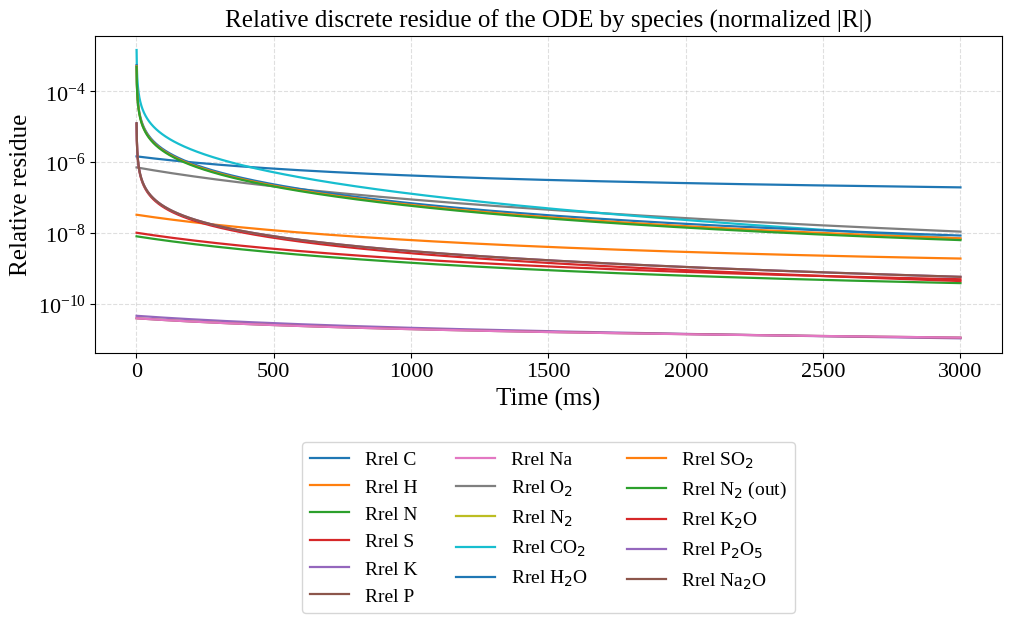
\includegraphics[width=\columnwidth]{FIGURES/residuals2.png}
    \caption{Relative discrete residue $|R|$ of each species over time, showing the decay of the normalized error until numerical stabilization and compliance with the $1.1\times10^{-3}$ convergence criterion.}

    \label{fig:residuals2}
\end{figure}

\textcolor{blue}{The convergence criterion applied to the model was established at a relative tolerance of $1\times10^{-4}$, as detailed in Section~\ref{Validation of the model}. To verify numerical stability, the discrete relative residue $|R|$ of each species concentration was monitored throughout the integration process. The results, presented in Figure~\ref{fig:residuals2}, show that after the convergence threshold was reached, the relative error continued to decrease monotonically until reaching stable values on the order of $10^{-8}$–$10^{-10}$. This confirmed that the propagation of numerical error was minimal and that the system reached a steady solution.  
Furthermore, the simulation was limited to 3000~ms because, within this period, all reactive species (particularly carbon) were completely consumed, consistent with the defined non-continuous fuel injection condition. Extending the simulation beyond this point would not alter the results, as the concentrations had already stabilized. \textit{We} think that the complete explanation makes unnecessary to show the residuals graphic as content of the paper. Nonetheless, we have strengthen the description of the error criterion convergence.\\}


Q4. Fig.5 same as Figs. 8 & 12, why heat released rapidly drop after AFR point?\\

\textcolor{blue}{
The explanation for this behavior has been clarified in the revised manuscript. The heat release shown in Figures~\ref{fig:PalmisteHeatAFR}, \ref{fig:EFBHeatAFR}, and \ref{fig:compAFR} is expressed per unit mass of the fuel--air mixture (kJ/kg). Once the AFR exceeds the stoichiometric value, the additional air does not contribute to the chemical energy released but instead increases the total mass of the mixture. This surplus air introduces mainly inert nitrogen and unreacted oxygen, which absorb part of the released heat and dilute the energy on a mass basis. As a result, the specific heat release decreases sharply beyond the stoichiometric point. This explanation has been incorporated into the discussion of Figure~\ref{fig:PalmisteHeatAFR}, with brief references added in the sections corresponding to Figures~\ref{fig:EFBHeatAFR} and~\ref{fig:compAFR}.}\\

Q5. Temperature is a key parameter of the combustion, but doesn’t present in this study?\\

\textcolor{blue}{The adiabatic flame temperature has been incorporated into the model, as now detailed in Section~\ref{energy_section}. Subsequently, the temporal evolution of this temperature has been evaluated to illustrate the total energy available in the system. As expected, the resulting values are relatively high because the analysis corresponds to an adiabatic condition, where no heat losses by radiation, conduction, or wall cooling are considered. Therefore, the results represent the upper thermal limit of the reaction, consistent with the kinetic model’s purpose of capturing the maximum theoretical energy release. This aspect is illustrated in Figures~\ref{fig:PalmisteHeatAFR} and~\ref{fig:EFBHeatAFR} at Sections~\ref{Heat release variation with AFR during PMF combustion} and \ref{Heat release variation with AFR during EFB combustion}.}
